\chapter{Diseño e Implementación}
\label{cap:capitulo4}

El objetivo de este \ac{TFG} es desarrollar un sistema de conducción autónoma capaz de realizar seguimiento de carril, control adaptativo al tráfico y maniobras de adelantamiento completas de manera segura en un entorno simulado. En este capítulo, se establecen primero los fundamentos de la percepción, definiendo qué elementos del entorno pueden ser detectados y qué información estará disponible para los modelos de control. A continuación, se explica el sistema implementado de conducción autónoma tradicional basado en el seguimiento de carril mediante un controlador \ac{PID}. Posteriormente, se exploran algunos algoritmos basados en \ac{DRL}) aplicados a la conducción autónoma, desarrollando y evaluando distintos modelos para la generación de comportamientos inteligentes. Finalmente, se lleva a cabo un análisis comparativo de los diferentes enfoques implementados, destacando sus ventajas e inconvenientes en el contexto de la conducción autónoma en un escenario urbano.

\section{Arquitectura general}

A continuación, se detalla la arquitectura general del sistema, ilustrada en la Figura \ref{fig:arch}, que consta de tres módulos principales. El vehículo en CARLA incluye los sensores y actuadores que permiten al sistema interactuar con el entorno. Entre los sensores el sistema dispone de cámaras RGB y \ac{LiDAR}, mientras que los actuadores cuentan con acelerador, giro y freno. La información captada por los sensores se transfiere al módulo de percepción para su procesamiento inteligente, cuyo objetivo es extraer información relevante y simplificada, que servirá como observaciones para los modelos de conducción autónoma. Por su parte, la cámara RGB permite la detección del carril y de la calzada, mientras que \ac{LiDAR} posibilita la detección de otros vehículos en la carretera. Finalmente, con este post-procesado el módulo de toma de decisiones es capaz de conseguir diferentes comportamientos autónomos basados en diversos algoritmos. Estas decisiones se aplican directamente en los actuadores del vehículo CARLA.

\begin{figure}[ht]
  \centering
  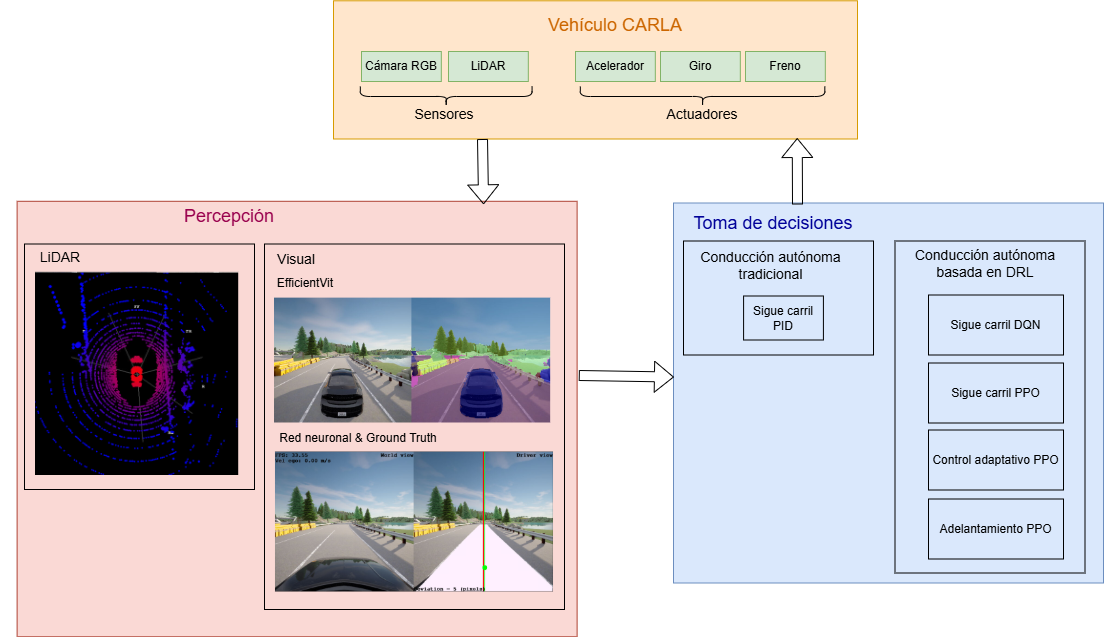
\includegraphics[width=16cm]{figs/Diseño/arquitectura.png}
  \caption{Arquitectura general.}
  \label{fig:arch}
\end{figure}

\section{Percepción visual}

La percepción visual es esencial para entender el entorno y tomar decisiones informadas en un sistema de conducción autónoma. Una habilidad básica de la que deben disponer este tipo de sistema es de la detección del carril que debe seguir. Para ir aún más allá, también se ha añadido un submodulo capaz de segmentar la calzada, lo que, por ejemplo, permite al sistema comprobar la existencia de otros carriles.

Las imágenes captadas por la cámara RGB del simulador CARLA tiene una resolución de 512 x 512 píxeles con un campo de visión de 90º, obtenido imágenes detallada con una perspectiva amplia. Esta cámara se coloca con una localización similar a la de un conductor. En esta sección, veremos cómo, a partir de esa información y aplicando diversas herramientas, es posible identificar el carril y segmentar la imagen.

\subsection{Detección del carril}

La detección del carril por el que debe circular nuestro vehículo autónomo es crucial para la toma de decisiones eficientes y seguras, garantizando que el vehículo no se desvíe a otros carriles o fuera de los límites de la carretera. Inicialmente, se usó el modelo basado en \ac{DL}, pero puesto que tiene cierta limitaciones imposibles de corregir, finalmente se terminó usando la técnica de \textit{ground truth}.

\subsubsection{Modelo basado en \ac{DL}}

El modelo de \ac{DL} para la detección de carril expuesto es la sección \ref{sec:carril_dl3} procesa imágenes de 512 x 1024 píxeles, mientras que las nuestra son de 512 x 512 píxeles. Por ello, primero creamos una imagen vacía y colocamos la imagen capturada por la cámara RGB en el centro. Esta imagen se pasa como entrada al modelo, el cual devuelve dos máscaras que definen las líneas del carril. En algunas situaciones, las líneas del carril pueden ser discontinuas o la red neuronal puede devolver líneas fragmentadas o incompletas. Dado que reentrenar la red no es una opción viable, aplicamos un proceso de post-procesado para mejorar la detección y obtener una línea continua y completa en toda la imagen, sin importar las condiciones. Para lograrlo, utilizamos regresión lineal sobre los puntos detectados de cada línea del carril. Este procedimiento nos permite calcular los coeficientes de las rectas que mejor se ajustan a esos puntos, y con ello, conocer sus límites de forma continua. Además, antes de aplicar la regresión lineal, se han aplicado técnicas de eliminación \textit{outliers} basadas en las medidas anteriores para lograr una detección aún más precisa del carril.

Una vez tenemos los coeficientes de las rectas que definen cada línea del carril, es muy sencillo calcular la coordenada \textit{x} de cada punto de la línea del carril dada la altura. Se ha definido una altura máxima para la detección del carril, creando así la forma de un trapecio como se puede observar en la Figura \ref{fig:dl_final_carril}. Al unir los puntos a la misma altura, podemos obtener el área del carril, su centro de masas y la desviación del coche con respecto al carril, considerando el centro de la imagen como el centro de nuestro vehículo. Además, podemos calcular \textit{n} puntos de cada línea del carril igualmente espaciados en el eje \textit{y} para terminar de conformar una representación simplificada de carril que, posteriormente, podrán recibir los modelos para la toma de decisiones.

\begin{figure}[ht]
\centering
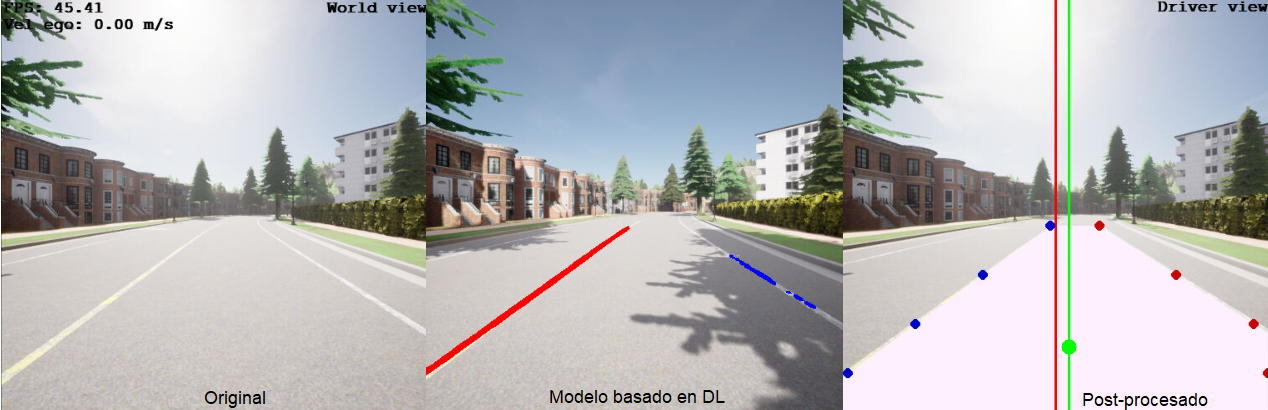
\includegraphics[width=14cm]{figs/Diseño/lane/lane_dl.png}
\caption{Detección de carril basada en \ac{DL}.}
\label{fig:dl_final_carril}
\end{figure}

Se ha implementado un sistema de memoria para filtrar mediciones erróneas. Este sistema almacena las cinco últimas detecciones de las líneas, junto con el ángulo que cada una forma con la horizontal. Si el ángulo de la detección actual difiere lo suficiente de la media de los ángulos almacenados o si no se detecta ninguna línea, descartamos la medida y utilizamos la última detección válida. Si esto ocurre durante más de cinco iteraciones consecutivas, determinamos que se ha perdido el carril.

A pesar de todos estos refinamientos en la detección de carril con \ac{DL}, cuando en la carretera hay un vehículo que obstruye la visibilidad de las líneas del carril, el modelo es incapaz de detectarlo de forma eficiente.

\begin{figure}[ht]
\centering
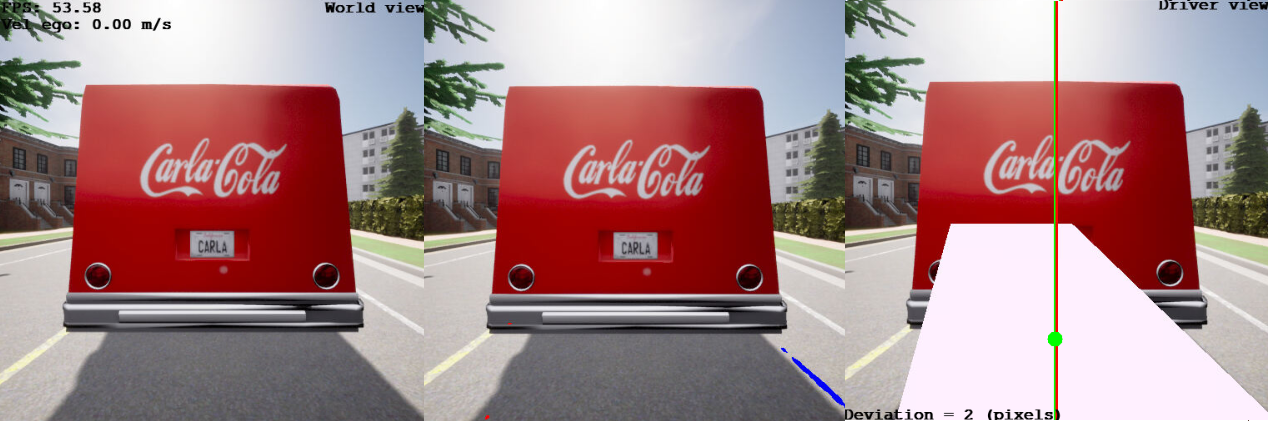
\includegraphics[width=14cm]{figs/Diseño/lane/lane_dl_obs.png}
\caption{Limitaciones de la detección de carril basada en \ac{DL}.}
\label{fig:dl_final_carril_obs}
\end{figure}

\subsubsection{Ground truth}

Si deseamos interactuar con otros vehículos en la carretera el modelo de detección de carril basado en \ac{DL} no es viable, por esta razón, surge la necesidad de utilizar \textit{ground thruth} para asegurar una detección del carril fiable en cualquier tipo de situación, incluso cuando la visibilidad es limitada. Una vez aplicada la técnica de \textit{ground thruth}, descrita en la sección \ref{sec:gt}, obtenemos algunos puntos del límites del carril, pero no todos. Para obtener los límites completos del carril, utilizamos la función \textit{pygame.draw.lines}. Sin embargo, esta función solo devuelve el rectángulo que rodea la línea dibujada, pero no los puntos de la línea en sí. Por lo tanto, dibujamos la línea sobre una superficie negra y luego analizamos esta superficie para localizar los límites del carril en términos de píxeles. Para optimizar el rendimiento computacional, restringimos la búsqueda al área dentro del rectángulo que encierra la línea. Al encontrar un punto, detenemos la búsqueda, ya que, dado que la línea es continua, podemos asumir con certeza que en cada altura habrá un punto que marcará el límite del carril. Si buscamos el límite izquierdo, comenzamos desde el inicio de la imagen (x = 0), mientras que, si buscamos el límite derecho, empezamos desde el final de la imagen. El siguiente código ilustra este proceso:

\begin{code}[h]
\begin{lstlisting}[language=Python]

rect = pygame.draw.lines(black_surface, (255, 0, 0), False, projected_boundary, 4)
pixels = []
for y in range(rect.top, rect.bottom):
    for x in range(start, end, step):
        color = black_surface.get_at((x, y))
        if color[0] == 255:
            pixels.append((x, y)) # Limits of the lane
            break
\end{lstlisting}
\caption[Identificación de puntos del carril con información de \textit{ground thruth}]{Identificación de puntos del carril con información de \textit{ground thruth}.}
\label{cod:gt_carril}
\end{code}

\newpage

De esta manera, obtenemos los límites de ambos lados del carril y aplicamos el mismo post-procesado que en el modelo basado en \ac{DL}, unimos los puntos a la misma altura para formar un trapecio y calcular las métricas del carril. 

\begin{figure}[ht]
\centering
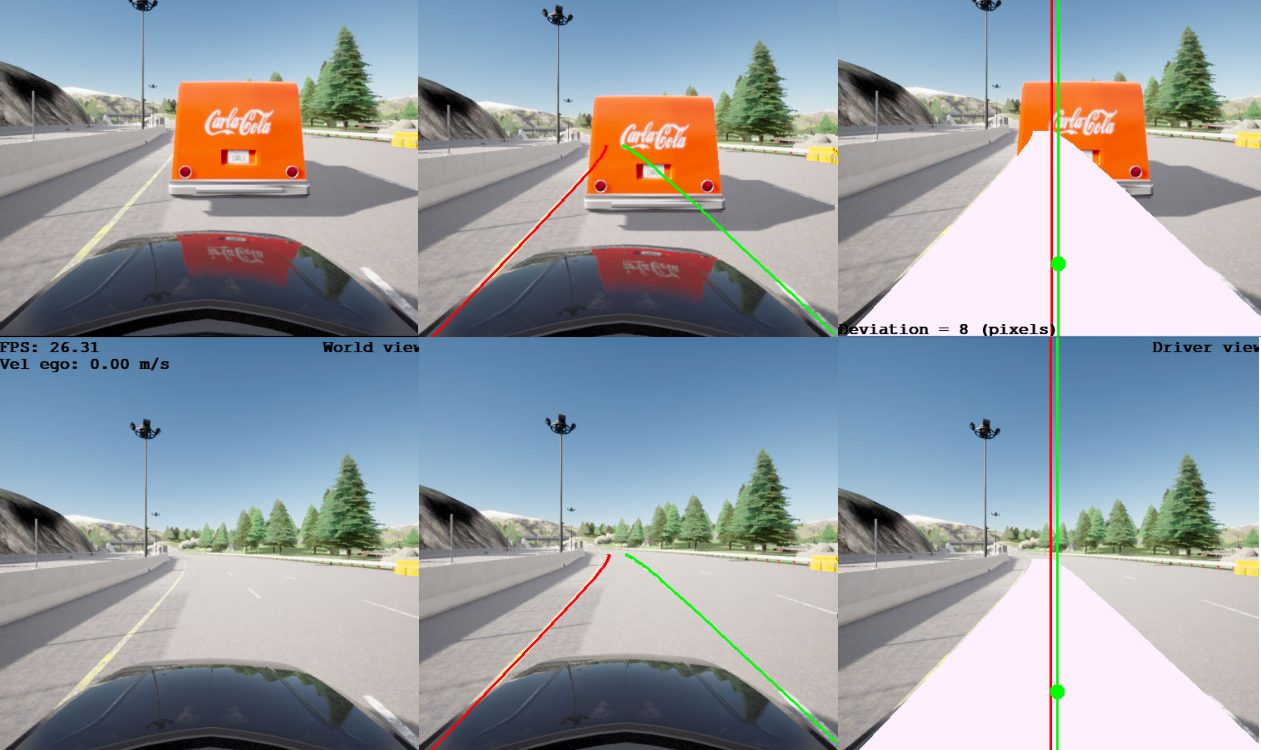
\includegraphics[width=13cm]{figs/Diseño/lane/ground_truth.png}
\caption{Detección de carril basada en \textit{ground thruth}.}
\label{fig:gt_final_carril}
\end{figure}

Al basarse en información obtenida directamente del simulador CARLA este enfoque resulta más fiable que la detección de carril mediante \ac{DL}, puesto que, a pesar de los posibles obstáculos que puedan afectar la visibilidad, es capaz de seguir detectando el carril como se muestra en la figura \ref{fig:gt_final_carril}. Por lo tanto, esta será la técnica empleada durante los entrenamientos, ya que, en ciertos escenarios, es necesario tener un vehículo delante que puede ocultar temporalmente las líneas del carril.

\subsection{Segmentación de la calzada}

Comprender la ubicación del carril por el que circulamos es fundamental, pero también buscamos obtener más información sobre la calzada: sus límites, su área y la presencia de otros carriles. Para ello, incluimos en la percepción de la red neuronal de segmentación semántica EfficientVit \ref{sec:ef}. Al igual que para el carril, necesitamos una representación simplificada de la misma, para ello, analizamos la máscara de segmentación que nos proporciona EfficientVit para calcular su área, centro de masas y \textit{n} puntos igualmente espaciados de cada límite lateral de la calzada. Con el fin proporcionar información más valiosa al modelo, seleccionamos solo un cuarto de los puntos de la parte totalmente vertical, como se puede apreciar en la Figura \ref{fig:seg_params}. Esta funcionalidad ha sido implementada principalmente con la librería NumPy para maximizar la eficiencia computacional.
\begin{figure}[ht]
\centering
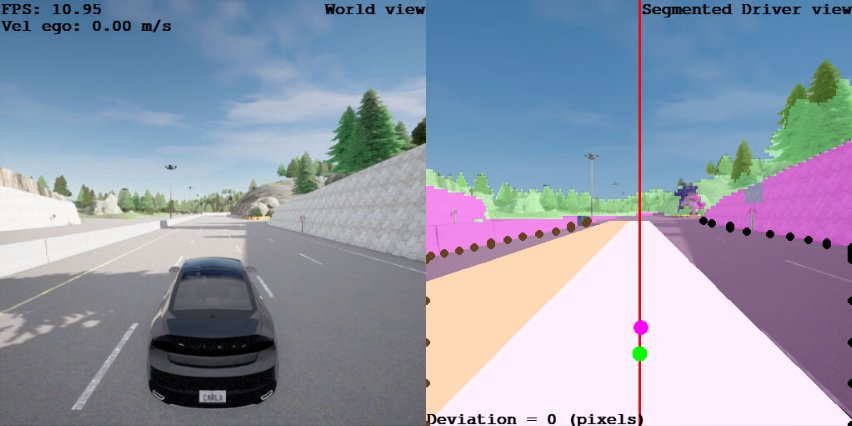
\includegraphics[width=10cm]{figs/Diseño/seg_points.png}
\caption{Representación de la calzada: superficie, centro de masas y límites.}
\label{fig:seg_params}
\end{figure}

También se utiliza la segmentación para comprobar el porcentaje del área del carril que es carretera y para saber si hay un carril a la izquierda. Esto nos proporciona más conocimiento acerca del entorno, lo que nos permitiría realizar maniobras como un adelantamiento, donde es necesario verificar la existencia de un carril al que podamos desplazarnos. Para hacer esta última comprobación, replicamos el carril actual a la izquierda y comprobamos que porcentaje de esta área es calzada, zona naranja en la Figura \ref{fig:seg_params}.

\section{Percepción basada en \ac{LiDAR}}

La percepción visual nos aporta mucha información sobre la calzada, pero también necesitamos detectar otros elementos que puede haber en la carretera. Para ello, añadimos un nuevo sensor a la percepción, el \ac{LiDAR}, que complementa la visión con datos precisos sobre obstáculos u otros vehículos que puedan aparecer durante la conducción. El \ac{LiDAR} es un sensor simulado de CARLA que proporciona como salida una nube de puntos que indica la distancia y la posición de los objetos en el entorno, permitiendo una reconstrucción de la escena para la percepción y navegación del vehículo autónomo. Se configura el \ac{LiDAR} con un alcance máximo de 20 metros, distancia suficiente para detectar obstáculos en la carretera, en nuestro caso otros vehículos. Para la representación gráfica de la información del \ac{LiDAR}, mostramos cada uno de los puntos de la nube en 2D, coordenadas \textit{x} e \textit{y}. Con el fin de mejorar la percepción visual, se ha interpolado el color de cada punto según su intensidad, siendo tonos rojos los valores más altos y azules los más bajos, y el tamaño según su altura, a mayor elevación mayor tamaño.

\begin{figure}[ht]
\centering
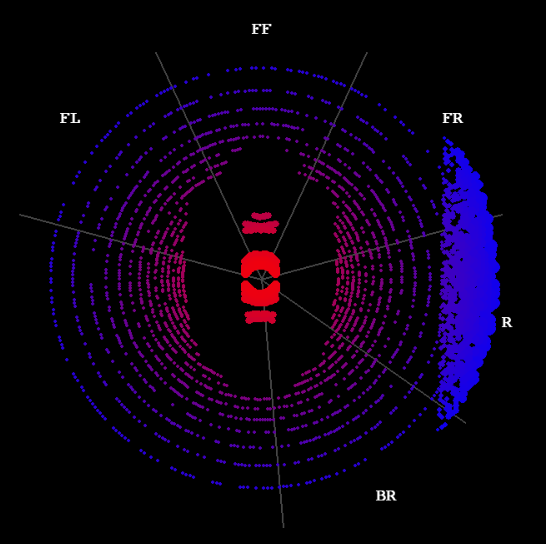
\includegraphics[width=10cm]{figs/Diseño/lidar/interpolate.png}
\caption{Visualización de la nube de puntos generada por el \ac{LiDAR}.}
\label{fig:interpolate_lidar}
\end{figure}

Para identificar vehículos en la trayectoria del vehículo, nos enfocamos en analizar la zona frontal del \ac{LiDAR} con una amplitud de 150º, dividida en tres subzonas de 50º: \textit{front-left}, \textit{front}, \textit{front-right}. Para determinar los ángulos que delimitan estas zonas independientemente de cómo se disponga el \ac{LiDAR} en el vehículo, debemos tener en cuenta la rotación del \ac{LiDAR} en el eje z (\textit{yaw}). Al ángulo deseado, la mitad de la zona frontal, le restamos el \textit{yaw} real y finalmente lo acotamos en un rango de [-180º, 180º]. Aunque ya hemos encontrado los ángulos extremos, es necesario calcular los dos ángulos intermedios que delimitan las tres zonas. Para ello, sumamos la amplitud de cada subzona al primer ángulo límite y se la restamos al segundo. Posteriormente, se incluyó la posibilidad de añadir dos nuevas subzonas en la parte lateral derecha del \ac{LiDAR}, \textit{right} y \textit{back-right}, permitiendo así la detección de obstáculos en un rango más amplio. En nuestro caso, con un \textit{yaw} de 90º, obtenemos los ángulos: [-165.0, -115.0, -65.0, -15.0, 35.0,  85.0].

\begin{code}[h]
\begin{lstlisting}[language=Python]
angle1 = get_angle_range(-self._front_angle / 2 - yaw)
angle2 = get_angle_range(self._front_angle / 2 - yaw)

angle1_add = get_angle_range(angle1 + self._front_angle / 3)
angle2_sub = get_angle_range(angle2 - self._front_angle / 3)        
self._angles = [angle1, angle1_add, angle2_sub, angle2]

if self._back:
	self._angles.append(angle2 + self._front_angle / 3)
	self._angles.append(angle2 + (self._front_angle / 3) * 2)
\end{lstlisting}
\caption[Cálculo de los ángulos de la zona del \ac{LiDAR}]{Cálculo de los ángulos del \ac{LiDAR}.}
\label{cod:angle_lidar}
\end{code}

\newpage

Como se puede observar en el dibujo \ref{fig:dib_angle}, dependiendo de que ángulo sea mayor, debemos seguir un criterio u otro para determinar si un punto pertenece o no la zona de interés o a una subzona concreta.
\begin{figure}[ht]
  \centering
  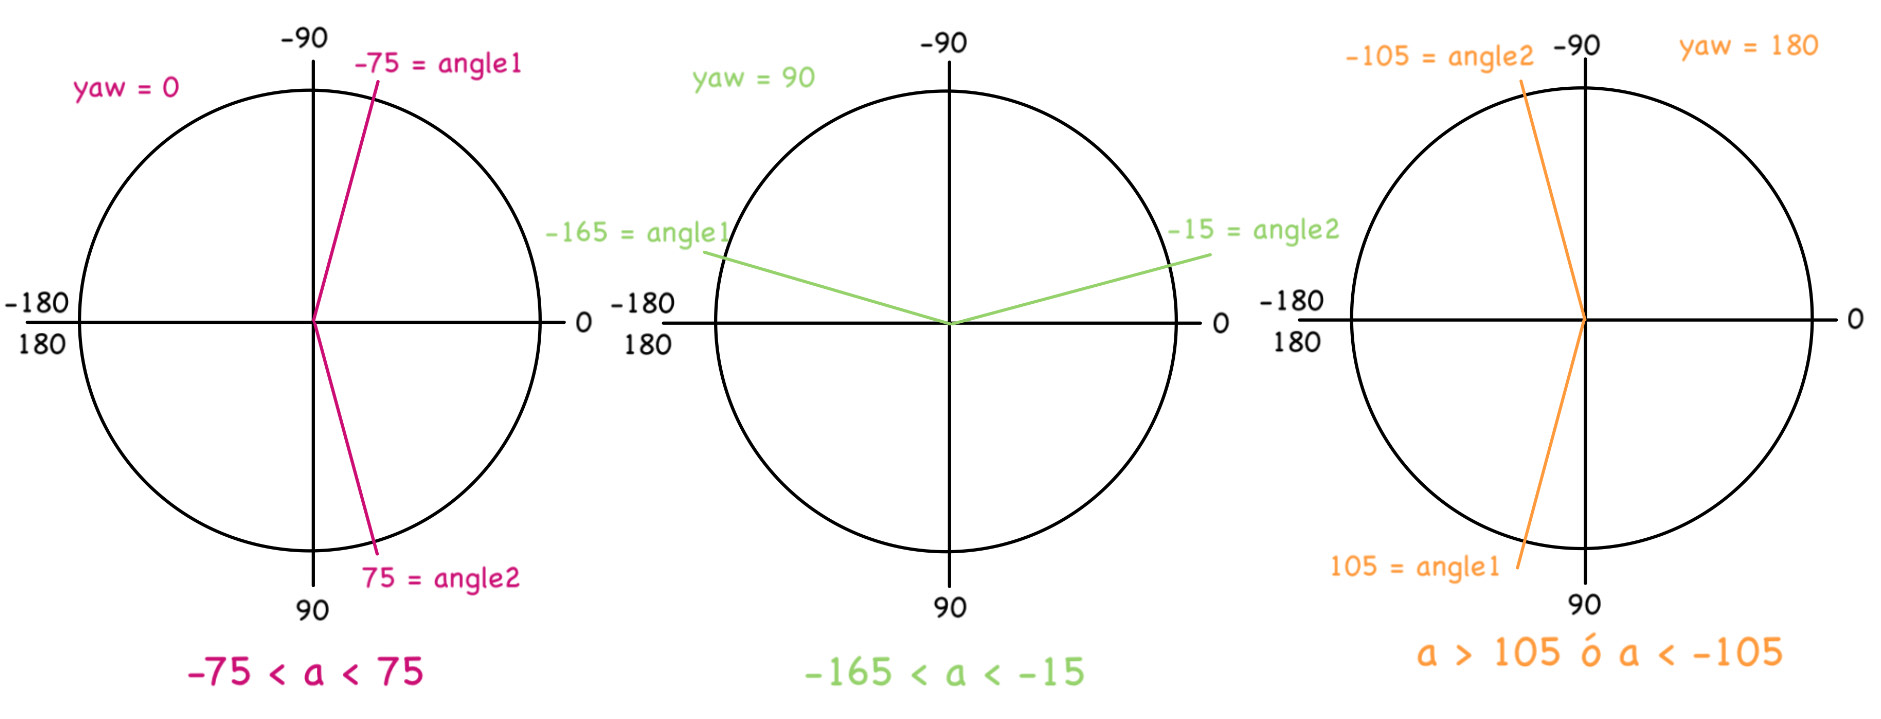
\includegraphics[width=10cm]{figs/Diseño/lidar/draw_angles.jpg}
  \caption{Criterio para saber a qué zona pertenece un punto del \ac{LiDAR}.}
  \label{fig:dib_angle}
\end{figure}

Para tener información adicional, se ha creado un cálculo de estadísticas para cada subzona: mínimo, media, mediana y desviación estándar. Como se puede observar en la Figura \ref{fig:stats_lidar}, los puntos de color rojo corresponden al propio coche, por lo tanto, hemos realizado un filtrado por intensidad para eliminarlos de los cálculos estadísticos. De la misma manera, filtramos por altura para eliminar todos los puntos correspondientes a la calzada y otros elementos del entorno externos a la carretera (montañas, árboles…), quedándonos solo con información relevante para la conducción.
\begin{figure}[ht]
  \centering
  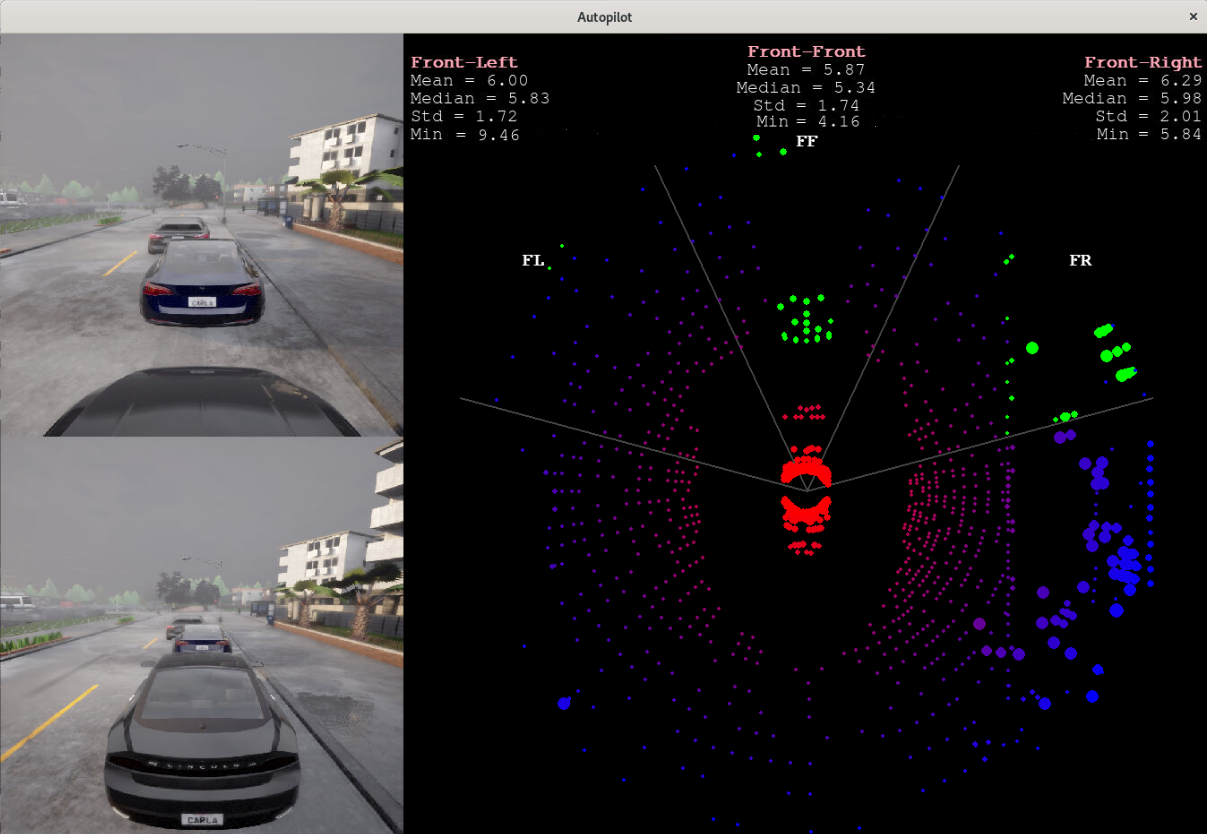
\includegraphics[width=11cm]{figs/Diseño/lidar/stats.png}
  \caption{Filtrado de puntos y cálculo de estadísticas del \ac{LiDAR}.}
  \label{fig:stats_lidar}
\end{figure}

\newpage

Se ha implementado una función que extrae un número determinado de puntos de cada subzona, los cuales están ordenados y distribuidos de manera equidistante a lo largo del eje \textit{x}. Estos puntos se utilizan como observaciones para los modelos, garantizando una representación precisa y bien estructurada de la información obtenida del \ac{LiDAR}.
\begin{figure}[ht]
\centering
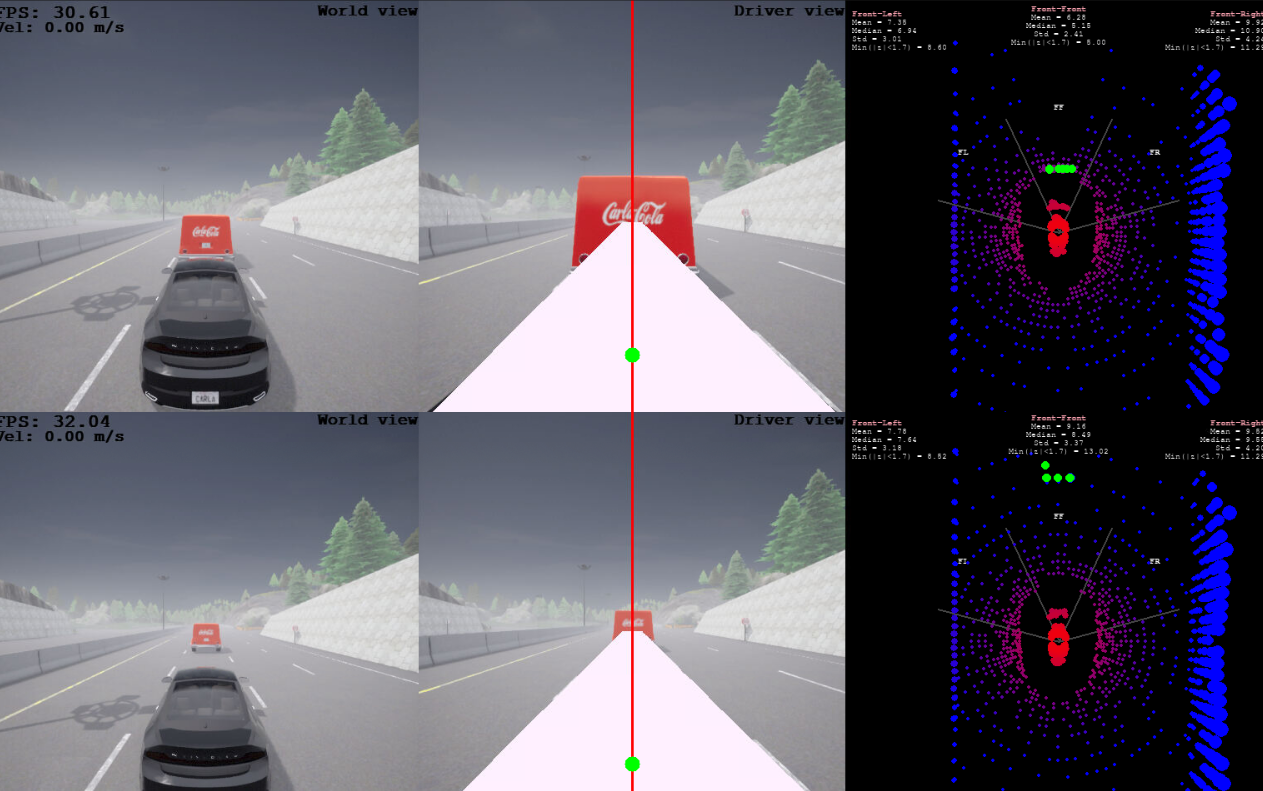
\includegraphics[width=12cm]{figs/Diseño/lidar/laser_front.png}
\caption{Selección de puntos de la subzona frontal del \ac{LiDAR}.}
\label{fig:laser_front}
\end{figure}

Se realizó un \textit{profiling} para evaluar las latencias y detectar los procesos con mayor consumo de tiempo en el código, con el objetivo de optimizar su eficiencia. Como se observa en la Figura \ref{fig:profiling}, la mayor parte del tiempo de cómputo se destina a la predicción con EfficientVit, mientras que el resto de los procesos presentan latencias acordes a su carga computacional y no suponen un inconveniente significativo. Tras analizar los resultados desde un enfoque tanto computacional como de desempeño, se ha concluido que la combinación de EfficientVit para la segmentación de la calzada, \textit{ground truth} para detección del carril y el \ac{LiDAR} como fuente adicional de datos para detectar obstáculos en la carretera, permite un equilibrio entre precisión y eficiencia de procesamiento. La latencia total de esta unión es de aproximadamente 93 ms, lo que en el simulador CARLA nos permite iterar a unos 10 \ac{FPS}. Este rendimiento es adecuado para aplicaciones en tiempo real, permitiendo así lograr comportamientos reactivos y robustos en dinámicos.
\begin{figure}[ht]
  \centering
  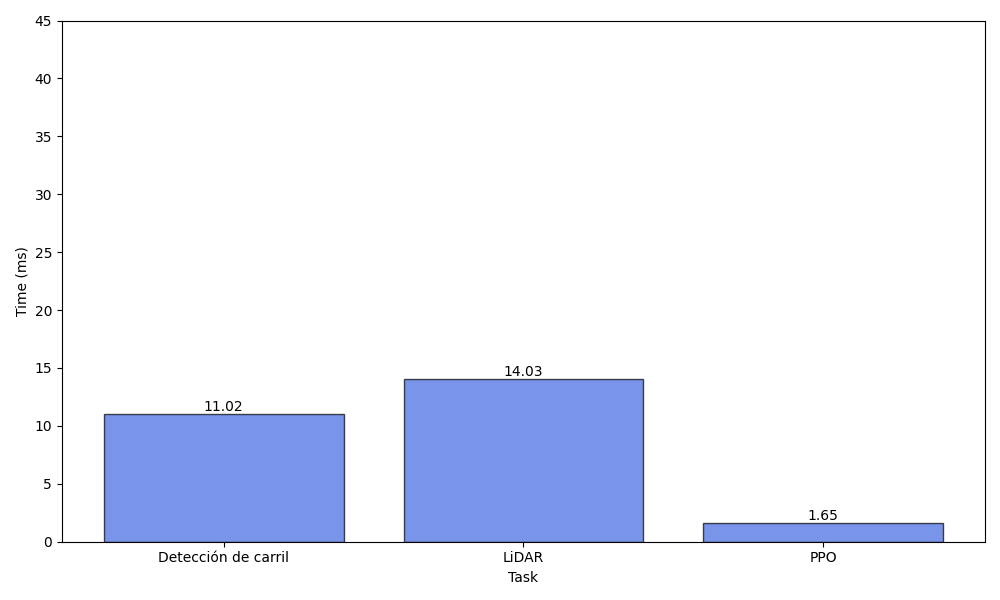
\includegraphics[width=7cm]{figs/Diseño/profiling.png}
  \caption{\textit{Profiling} del proceso de percepción.}
  \label{fig:profiling}
\end{figure}

\section{Toma de decisiones}

El módulo de toma de decisiones permite a nuestro sistema interpretar el entorno de manera eficiente según los datos procedentes de percepción. Un sistema de conducción autónoma debe ser capaz de adaptarse a escenarios complejos y cambiantes, con variaciones en la dirección del carril, el número de carriles o el comportamiento de los demás vehículos en la carretera. Debe ser capaz de tomar decisiones informadas, seguras y óptimas, asegurando comportamientos realistas, evitando accidentes y respetando las normativas de tráfico en todo momento.

La información procesada por los sensores puede interpretarse de diversas formas para la toma decisiones informadas. Existen métodos más tradicionales basados en reglas predefinidas y sistemas matemáticos, así como enfoques más avanzados basados en \ac{ML}. Sin embargo, una toma de decisiones rígida, basada en reglas fijas y algoritmos deterministas, no es adecuada para situaciones reales, donde la incertidumbre es un factor clave. En estos casos, necesitamos modelos capaces de adaptarse a escenarios cambiantes. Si se quisieran utilizar modelos matemáticos complejos y muy detallados del vehículo y del entorno, lo que podría generar una carga computacional excesiva. Por otro lado, el \ac{ML} permite gestionar esta información de forma más eficiente, adaptándose a las variaciones en el entorno y mejorando el rendimiento del sistema.

Para la conducción autónoma basada en \ac{ML}, nos centraremos en el aprendizaje por refuerzo, descrito en la primera sección \ref{sec:refuerzo}. Como se ha comprobado en anteriores \ac{TFG}\footnote{\url{https://burjcdigital.urjc.es/items/f6ce4e69-199b-4f73-a136-0f4782eac351}} que han empleado este enfoque, en particular \textit{Q-learning}\footnote{\url{https://www.cs.us.es/~fsancho/Blog/posts/Aprendizaje_por_Refuerzo_Q_Learning.md}}, un algoritmo basado en tablas, presenta ciertas limitaciones que dificultan su escalabilidad para nuestro objetivo. Cuando los estados y las acciones son continuos o muy numerosos, como ocurre en nuestro escenario de conducción autónoma, no es práctico utilizar una tabla para almacenar los valores de las acciones, ya que sería necesario explorar cada estado al menos una vez para encontrar la solución más óptima. 

Por ello, en este \ac{TFG} se ha empezado directamente con algoritmos basados en \ac{DRL}. En su lugar, estos algoritmos redes neuronales diseñadas para aprender la función que mapea estados-acciones. Estas redes son capaces de estimar el valor de estados, ya que aprende las relaciones entre los diferentes pares estado-acción, permitiéndole generalizar de manera más eficiente, mejorar su rendimiento en entornos complejos donde las reglas no son evidentes y adaptarse a nuevas situaciones sin necesidad de explorar cada estado de forma explícita. Por ejemplo, aunque hayan sido entrenadas con curvas de 30º o menos, los modelos resultantes son capaces de generalizar y tomar adecuadamente una curva de 40º. En este \ac{TFG} se han utilizado los algoritmos de \ac{DQN} y \ac{PPO}. 

\subsection{Conducción autónoma tradicional basada en un controlador \ac{PID}}

A pesar de no ser la solución más óptima, existen técnicas de control clásico que funcionan adecuadamente para ciertas habilidades de conducción. Un controlador \ac{PID} es un tipo de control ampliamente utilizado en sistemas automáticos para ajustar una variable y mantenerla en un valor deseado. En conducción autónoma, se usa para mantener un vehículo en el carril ajustando el ángulo del volante según la desviación del carril.

Para el seguimiento de carril basado en un controlador tradicional\footnote{\url{https://youtu.be/mq5STc8-Z6Y}}, se ha implementado un controlador PD para controlar el giro. Al mismo tiempo, el acelerador se mantiene fijo a 0.5, mientras que con el freno regula la velocidad para mantenerla constante a aproximadamente 10 m/s.
\begin{code}[h]
\begin{lstlisting}[language=Python]
self._kp = 1 / (SIZE_CAMERA / 2)
self._kd = -self._kp / 1.7
self._throttle = 0.5
\end{lstlisting}
\caption[Definición de constantes para el controlador \ac{PID}]{Definición de contantes para el controlador \ac{PID}.}
\label{cod:const_pid}
\end{code}

En el módulo de percepción, ya hemos calculado la desviación respecto al centro del carril del vehículo. Esta desviación representa el error que recibe nuestro controlador. El componente proporcional se encarga de normalizar el error en el rango de giro, mientras que el signo del error ya indica el sentido del giro. Si el error supera cierto umbral, lo incrementamos ligeramente para mejorar el rendimiento en las curvas. El componente derivativo evita movimientos oscilatorios al salir de las curvas, ya que resta el error anterior reducido. Este componente resta el valor del error anterior, pero solo lo consideramos si su signo es diferente al del error actual, ya que, de lo contrario, podría causar inestabilidad y afectar negativamente la conducción durante las curvas.
\begin{code}[h]
\begin{lstlisting}[language=Python]
# Different sign
if (self._error > 0 and self._prev_error < 0) or (self._error < 0 and self._prev_error > 0):
    self._prev_error = 0       

# Increase in error
if error > 20:
    error *= 1.15

control.steer = self._kp * error + self._kd * self._prev_error
\end{lstlisting}
\caption[Regulación del giro mediante el controlador \ac{PID}]{Regulación del giro mediante el controlador \ac{PID}.}
\label{cod:pid_giro}
\end{code}

En los histogramas \ref{fig:comparativa_pid}(a) se muestra la velocidad en m/s del coche autónomo y el error respecto al centro del carril en píxeles durante el circuito en el que se ajustó el controlador \ac{PID}, mientras que en los histogramas \ref{fig:comparativa_pid}(b) se presenta la misma información, pero para un circuito en el que no se realizó el ajuste. Cabe destacar que este último circuito cuenta con dos curvas pronunciadas a la derecha. En ambos casos, podemos ver que el coche acelera al inicio, alcanzando rápidamente una velocidad de 10 m/s, la cual se mantiene constante durante todo el recorrido. Aunque en ambos escenarios el histograma de la desviación está bastante centrado, en el circuito sin ajuste, se observan desviaciones muy elevadas, superiores a 30 píxeles, con una frecuencia considerable. A pesar de las curvas acentuadas, estas desviaciones no deberían ser tan altas, puesto que el vehículo debería mantenerse dentro de los límites del carril para garantizar una conducción segura y eficiente. Esto sugiere que un controlador \ac{PID} no es capaz de generalizar adecuadamente ante carriles cambiantes, provocando inestabilidad en la trayectoria y en el comportamiento del vehículo.

\begin{figure}[ht]
  \centering
  \subfigure[Histogramas del circuito ajustado.]{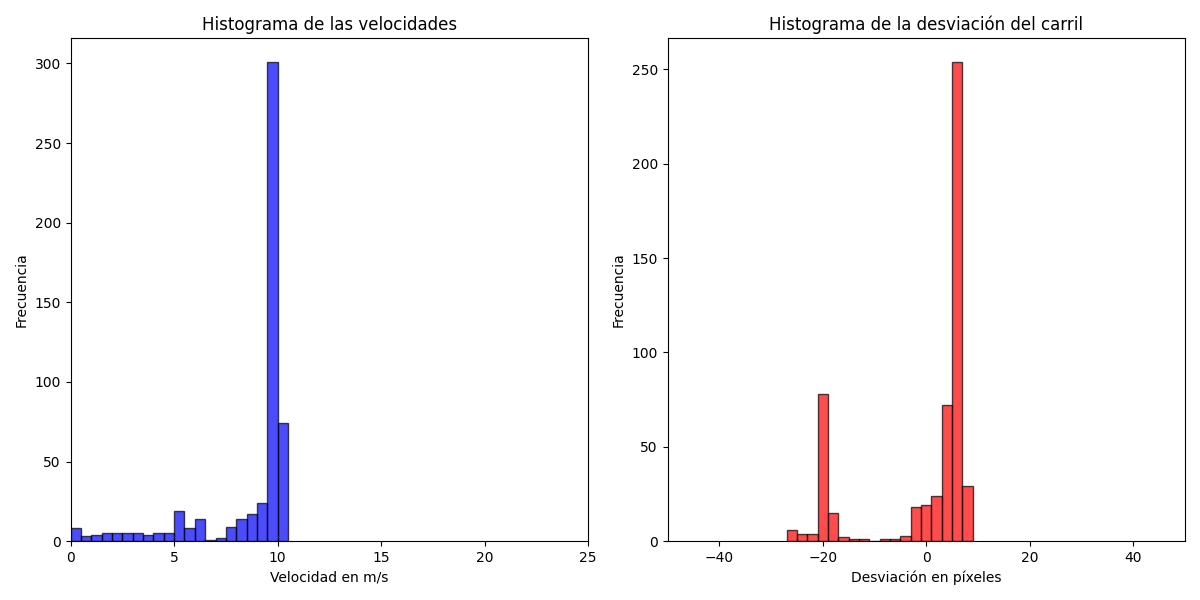
\includegraphics[width=0.45\textwidth]{figs/Diseño/pid/escenario_ajustado.png} \label{fig:pid_ajus}}
  \hfill
  \subfigure[Histogramas del circuito no ajustado.]{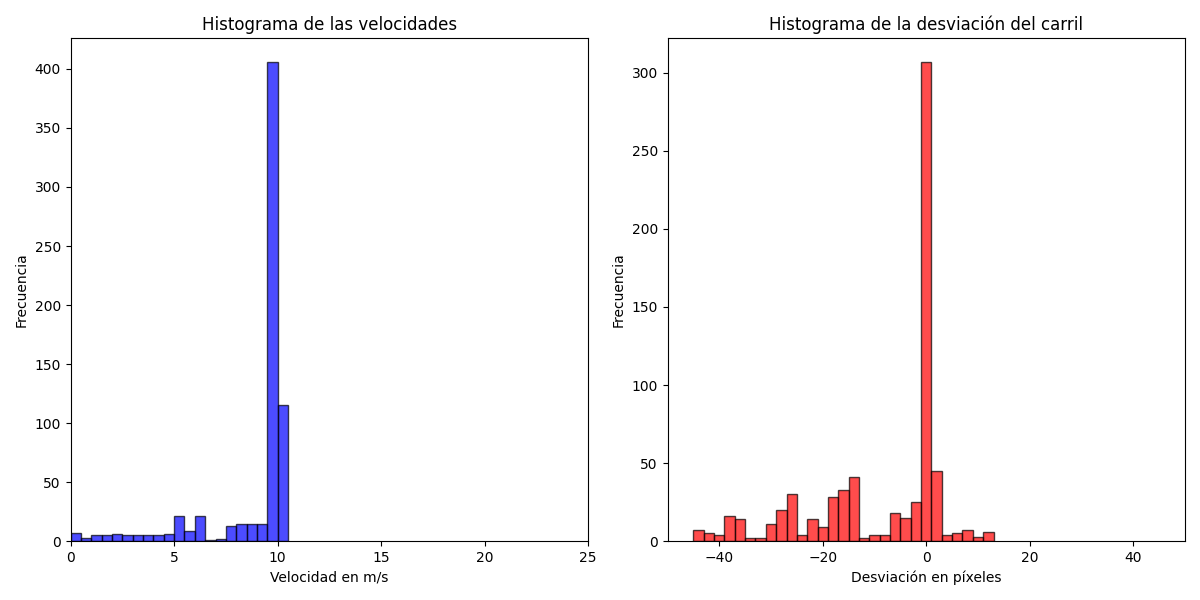
\includegraphics[width=0.45\textwidth]{figs/Diseño/pid/escenario_no_ajustado.png} \label{fig:pid_no_ajus}}
  \caption{Comparativa de la velocidad y desviación del vehículo en dos escenarios: con y sin ajuste del controlador \ac{PID}.}
\label{fig:comparativa_pid}
\end{figure}

\subsection{Seguimiento de carril con \ac{DQN}}

Como se describió en la sección \ref{sec:stable_baselines3}, \ac{DQN} es un algoritmo \textit{off policy} que permite un espacio de observaciones continuo, pero discreto de acciones. Ahora que ya sabemos cómo funciona el algoritmo \ac{DQN}, llega la hora de construir el entorno de entrenamiento para que un coche autónomo sea capaz de seguir el carril. Primero, debemos elegir el circuito de entrenamiento para nuestro modelo, para ello, hemos elegido el Town04 de CARLA, ya que incluye tramos largos y sin intersecciones. Como se muestra en la Figura \ref{fig:mapa}, se han definido cuatro rutas: las rutas uno, dos y tres, representadas por los colores rosa, amarillo y \textit{aqua} respectivamente, se utilizan durante el entrenamiento, mientras que la ruta cuatro, en color azul, se emplea para examinar el modelo en inferencia y comprobar si es capaz de generalizar. Cada una de estas rutas de entrenamiento comienza en una dirección y punto distinto: curva a la derecha, línea recta y curva a la izquierda, con el fin de evitar \textit{overfitting} en el modelo.

\begin{figure}[ht]
  \centering
  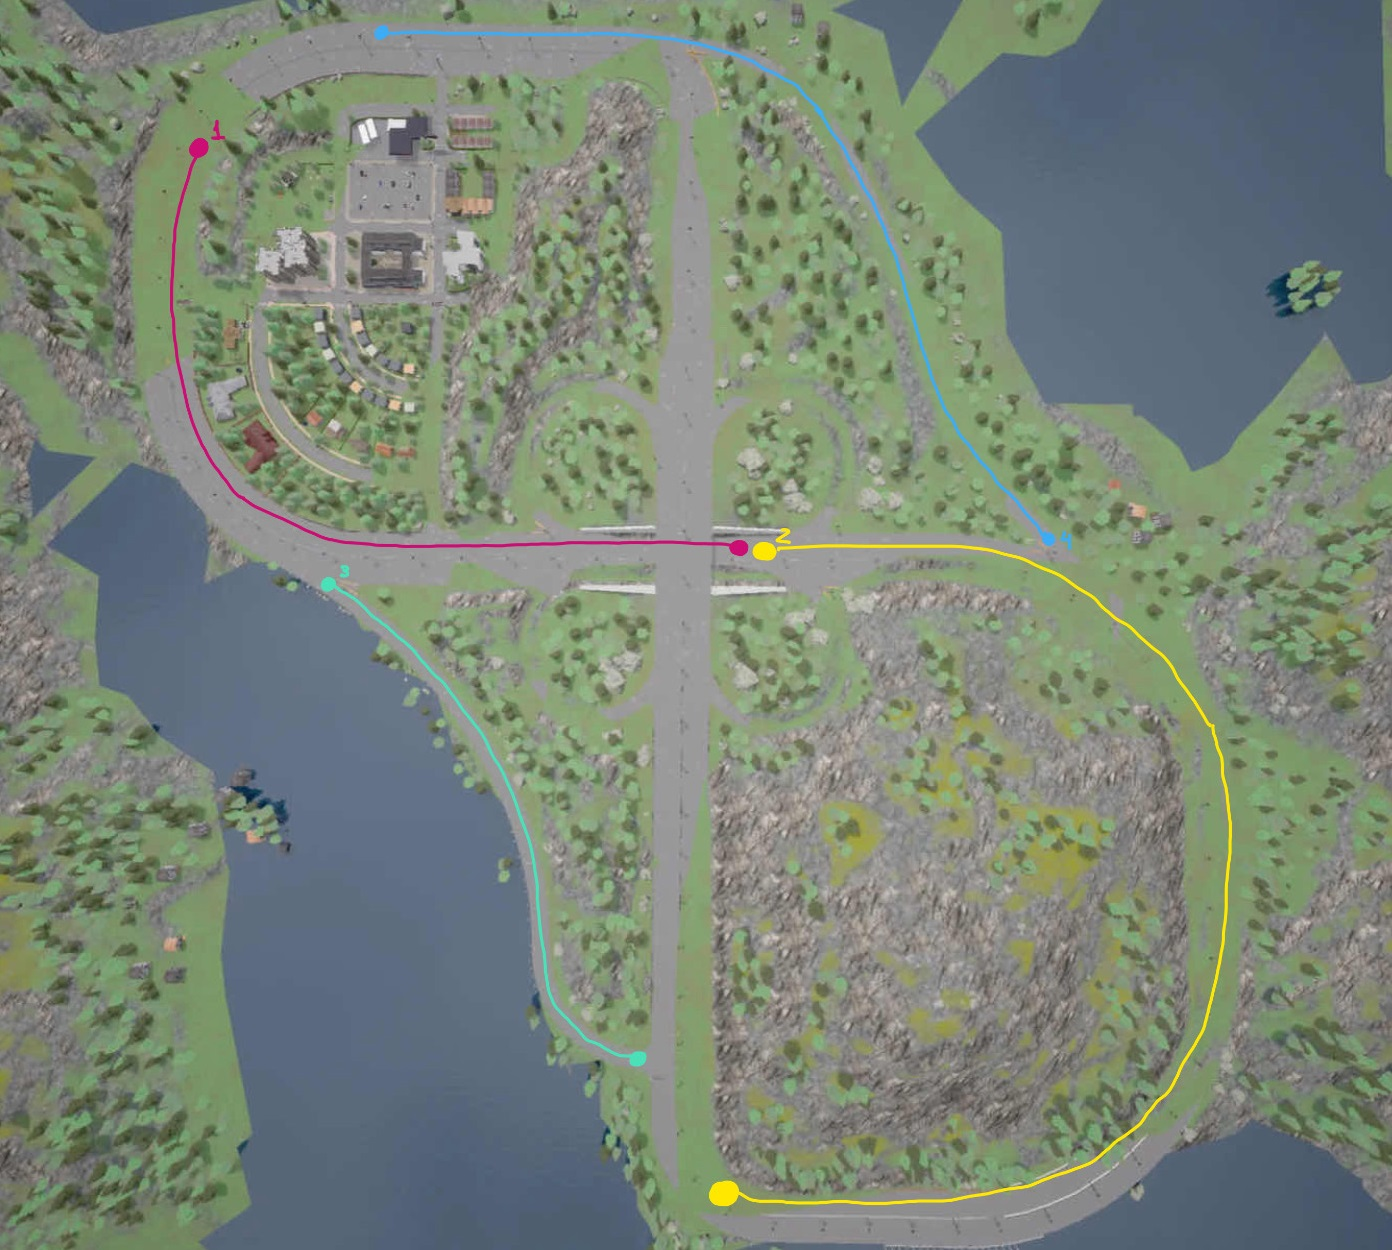
\includegraphics[width=8cm]{figs/Diseño/mapa.jpeg}
  \caption{Mapa del entorno de entrenamiento en CARLA con rutas definidas.}
  \label{fig:mapa}
\end{figure}

\newpage

El espacio de observaciones coincide con el espacio de estados y está basado en un diccionario, por lo tanto, empleamos la política \textit{MultiInputPolicy} \ref{sec:stable_baselines3}. Las observaciones se normalizan para facilitar el aprendizaje al modelo e incluyen la siguiente información: 
\begin{itemize}
		\item Desviación del carril.
		\item Área del carril.
		\item Cinco puntos de la línea izquierda del carril.
		\item Cinco puntos de la línea derecha del carril.
		\item Centro de masas.
\end{itemize}

\begin{figure}[ht]
  \centering
  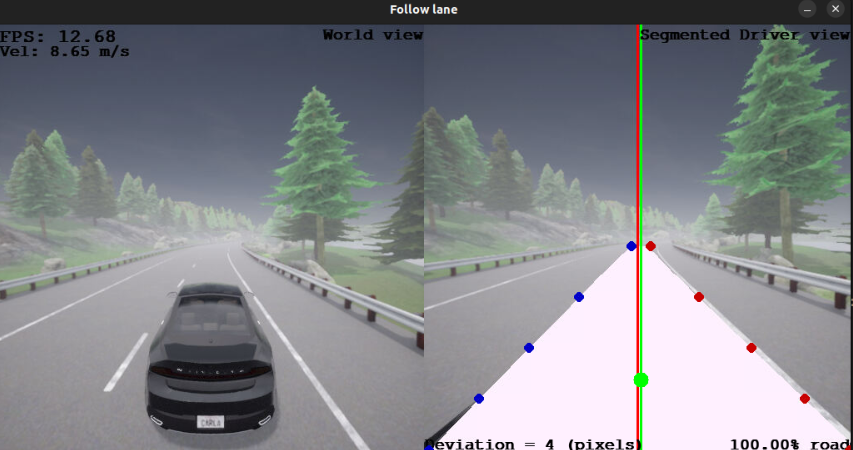
\includegraphics[width=8cm]{figs/Diseño/discrete/obs_dqn.png}
  \caption{Observaciones seguimiento de carril basado en \ac{DQN}.}
  \label{fig:dqn_obs}
\end{figure}

Como hemos mencionado al inicio, \ac{DQN} permite un espacio de acciones discreto. Las acciones están compuestas por un comando de acelerador y otro de giro, para combinarlo hemos seguido la regla de que, a mayor aceleración, menor es el giro. En total, se han definido 21 acciones disponibles entre las cuales el coche autónomo podrá seleccionar aquellas que maximicen la recompensa en cada situación.

\begin{code}[h]
\begin{lstlisting}[language=Python]

self.action_to_control = {
    0: (0.5, 0.0),
    1: (0.45, 0.01), 
    2: (0.45, -0.01),
    3: (0.4, 0.02),
    4: (0.4, -0.02),
    5: (0.4, 0.04),
    6: (0.4, -0.04),
    7: (0.4, 0.06),
    8: (0.4, -0.06),
    9: (0.4, 0.08),
    10: (0.4, -0.08),
    11: (0.3, 0.1),
    12: (0.3, -0.1),
    13: (0.3, 0.12),
    14: (0.3, -0.12),
    15: (0.2, 0.14),
    16: (0.2, -0.14),
    17: (0.2, 0.16),
    18: (0.2, -0.16),
    19: (0.1, 0.18),
    20: (0.1, -0.18)
}
\end{lstlisting}
\caption[Acciones disponibles para el seguimiento de carril basado en \ac{DQN}]{Acciones disponibles para el seguimiento de carril basado en \ac{DQN}.}
\label{cod:acc_dqn}
\end{code}

Nuestro objetivo es que el coche circule por el centro del carril sin desviarse, manteniendo una conducción fluida y a velocidades considerables. Para lograrlo, hemos diseñado una función de recompensa que se basa principalmente en la desviación del carril y en la velocidad actual del coche, normalizando y ponderando estos valores según sus respectivos pesos. Sin embargo, si el coche colisiona contra un elemento del entorno (sensor de colisión \ref{sec:carla}), pierde o cambia de carril, el episodio se detiene y se asigna una recompensa negativa.

\begin{code}[h]
\begin{lstlisting}[language=Python]
if error == None:
      # Clip deviation and velocity
      r_dev = (MAX_DEV - abs(np.clip(self._dev, -MAX_DEV, MAX_DEV))) / MAX_DEV
      r_vel = np.clip(self._velocity, 0.0, self._max_vel) / self._max_vel
      reward = 0.8 * r_dev + 0.2 * r_vel
else:
      reward = -30
\end{lstlisting}
\caption[Función de recompensa sigue-carril basado en \ac{DQN}]{Función de recompensa sigue-carril basado en \ac{DQN}.}
\label{cod:rew_dqn}
\end{code}

Durante los entrenamientos utilizamos el modo síncrono de CARLA, en el cual el cliente puede indicar al servidor cuándo ejecutar \textit{world.tick()} y durante cuánto tiempo simulado debe hacerlo \textit{fixed\_delta\_seconds}, luego detiene la simulación hasta que se llama de nuevo a \textit{tick}. Hemos utilizado un \textit{fixed\_delta\_seconds} de 50ms en CARLA, lo que equivale a entrenar a 20 \ac{FPS}, por lo tanto, en inferencia necesitamos operar al menos a esta velocidad. Los entrenamientos tuvieron una duración de 26 horas. Tras realizar diversas pruebas experimentales, identificamos los hiperparámetros de entrenamiento que proporcionan los mejores resultados.
\begin{table}[ht]
\centering
\begin{tabular}{|l|l|l|}
\hline
\textbf{Hiperparámetro} & \textbf{Valor} & \textbf{Descripción} \\ \hline
learning\_rate & 0.0005 & Tasa de aprendizaje \\ \hline
buffer\_size & 20,000 & Tamaño de la memoria (\textit{replay memory}) \\ \hline
batch\_size & 1024 & Tamaño del lote \\ \hline
gamma & 0.85 & Factor de descuento: importancia de las recompensas futuras frente a las inmediatas \\ \hline
target\_update\_interval & 1024 & Intervalo de actualización de la red neuronal objetivo \\ \hline
train\_freq & 256 & Frecuencia de entrenamiento: cada cuantos pasos de actualiza la red neuronal \\ \hline
gradient\_steps & 2 & Pasos de gradiente en cada actualización \\ \hline
exploration\_fraction & 0.8 & Fracción de exploración \\ \hline
exploration\_final\_eps & 0.0 & Valor final de exploración \\ \hline
n\_timesteps & 8,000,000 & Número total de steps \\ \hline
\end{tabular}
\caption{Hiperparámetros de entrenamiento en \ac{DQN} y sus valores.}
\label{tab:hiperparametros}
\end{table}

La frecuencia de entrenamiento resultó ser un factor clave en el proceso, al principio se utilizó un valor menor, pero los modelos no lograban converger. Esto se debe a que, al actualizar el modelo con ejemplares demasiado consecutivos, los datos están altamente correlacionados, generando inestabilidad y dificultando la convergencia. Sin embargo, al aumentar el valor de este hiperparámetro, la memoria acumula datos más diversos y significativos antes de actualizar el modelo.

En la gráfica \ref{fig:train_dqn}, se puede observar cómo el modelo finalmente converge. El primer \textit{plot} muestra la recompensa obtenida en cada episodio (azul) y recompensa promedio acumulada por episodio (amarillo), que finalmente se estabiliza en un valor de 3.500 aproximadamente. En el segundo \textit{plot} se muestra el número de \textit{steps} por episodio. A pesar de que al inicio los episodios son más largos y, po lo tanto, acumulan una mayor recompensa, no es ese el comportamiento que deseamos. A pesar de que al inicio los episodios son más largos y, por lo tanto, acumulan una mayor recompensa, no es el comportamiento que deseamos. Buscamos que el modelo alcance velocidades significativas, por lo que, a medida que aprende, los episodios tienen menos \textit{steps}, logrando completar el circuito más rápido sin comprometer la eficiencia. Los puntos verdes indican que el agente ha sido capaz de completar con éxito, mientras que los rojos señalan que ha tomado una acción que ha provocado el fin del episodio, como salirse del carril. Finalmente, en el último \textit{plot} se muestra cómo evoluciona el ratio de exploración, su valor se reduce gradualmente durante el 80\% del entrenamiento y, a partir de ese punto, se dejan de realizar acciones aleatorias.
\begin{figure}[ht]
  \centering
  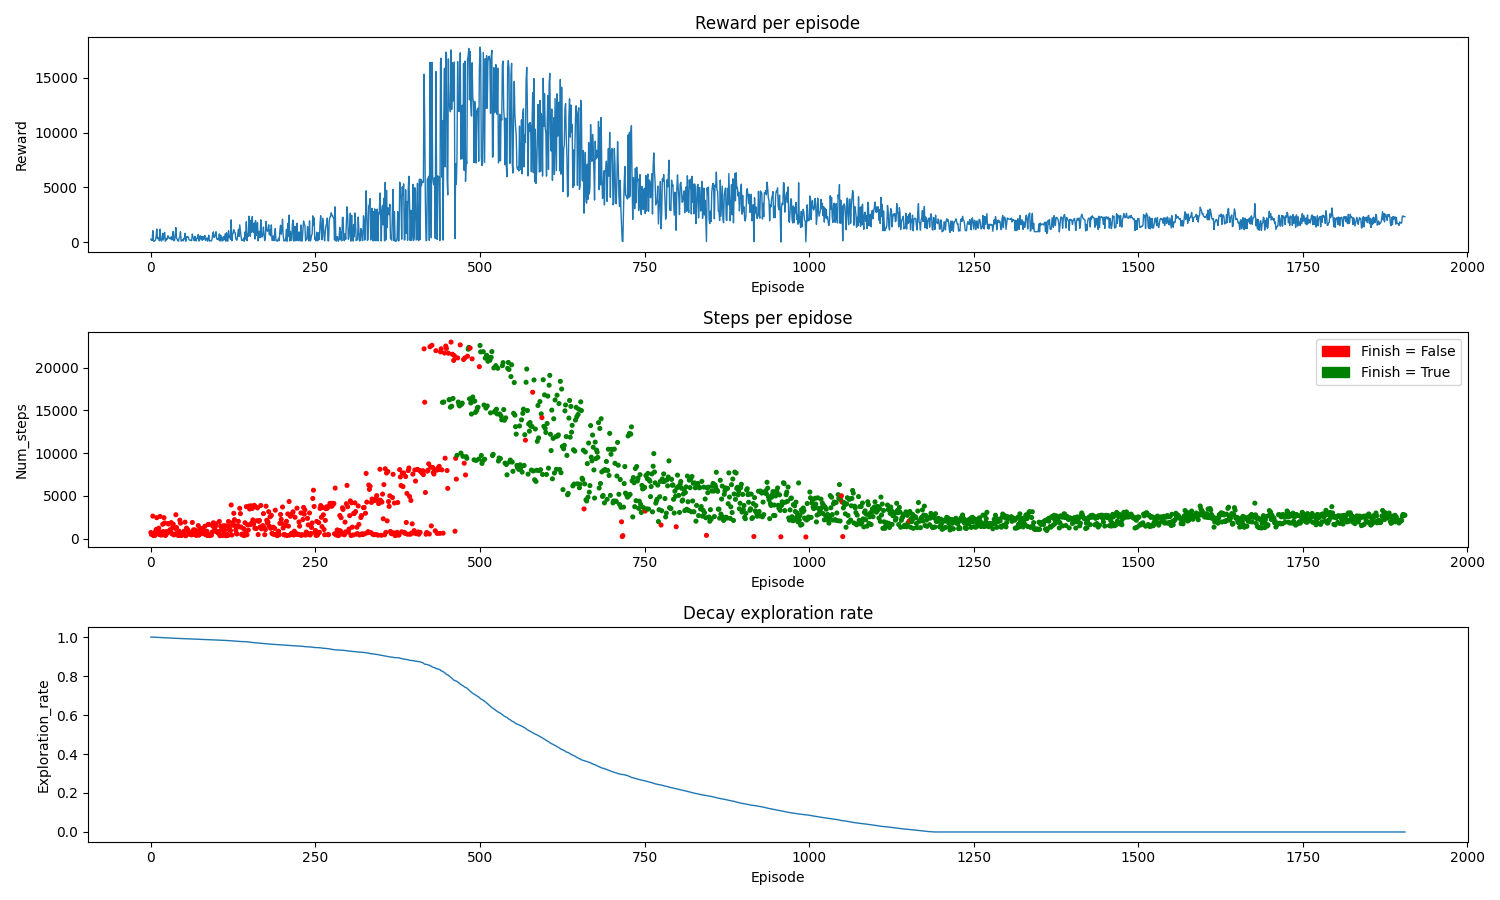
\includegraphics[width=13cm]{figs/Diseño/discrete/train_dqn.png}
  \caption{Gráfica de entrenamiento sigue-carril basado en \ac{DQN}.}
  \label{fig:train_dqn}
\end{figure}

En inferencia, usamos el modo asíncrono de CARLA, permitiendo que el simulador ejecute a la máxima velocidad posible. En un circuito visto durante el entrenamiento\footnote{\url{https://youtu.be/rzy2Vg57zA8}}, se observa que el seguimiento del carril es bastante preciso, no obstante, ocasiones, se percibe un pequeño balanceo. Esto se debe a una de las limitaciones de \ac{DQN}, su espacio de acciones es discreto no permite seleccionar la acción de giro óptima en cada momento. En la Figura \ref{fig:inference_dqn}, se presentan las acciones tomadas durante inferencia. Los histogramas indican mayoritariamente se eligen los pares de acciones más rápidos y giros más suaves, llegando a alcanzar una velocidad de 50 km/h.
\begin{figure}[ht]
  \centering
  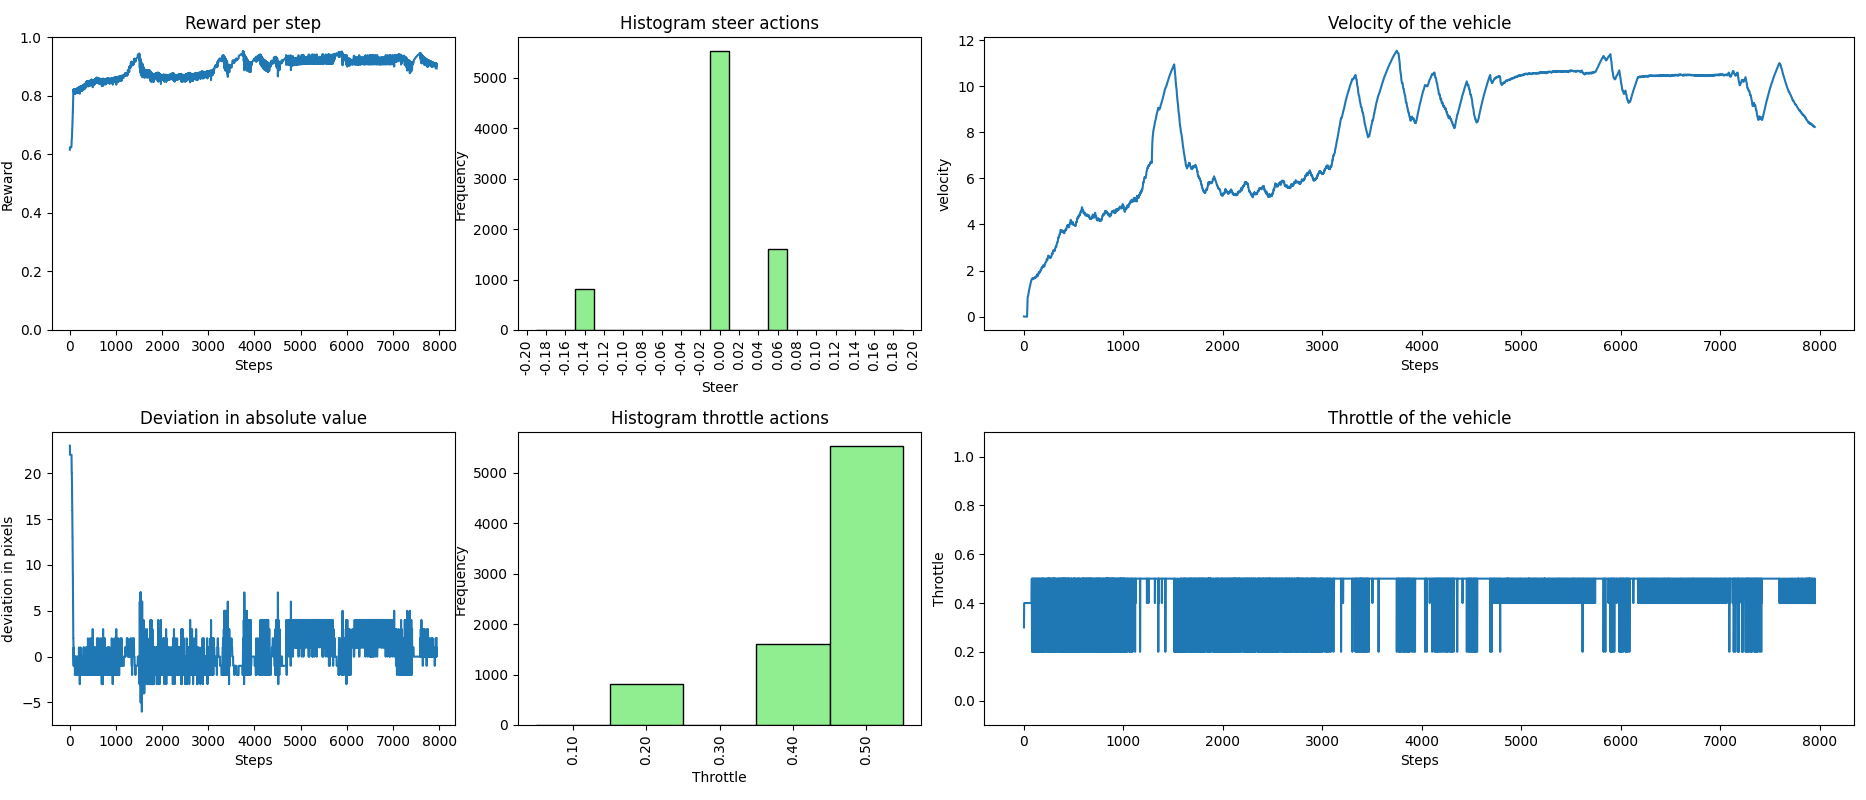
\includegraphics[width=10cm]{figs/Diseño/discrete/inference_dqn.png}
  \caption{Gráficas de inferencia sigue-carril basado en \ac{DQN}.}
  \label{fig:inference_dqn}
\end{figure}

En la Figura \ref{fig:comparativa_dqn}, se muestra la velocidad del coche autónomos en m/s y el error al centro del carril en píxeles del modelo basado en \ac{DQN}, comparando un escenario visto durante el entrenamiento, el mostrado en el vídeo, con otro circuito no visto previamente. En ambos casos, el histograma referente a la desviación del carril se mantiene concentrado en el centro, lo que indica que el modelo es capaz de seguir el carril de forma precia. Sin embargo, el histograma de la velocidad se desplaza hacia la izquierda, evidenciando un comportamiento más lento y un modelo con dificultades para generalizar en nuevos entornos.
\begin{figure}[ht]
\centering
\subfigure[Histogramas de un circuito visto durante el entrenameinto.]{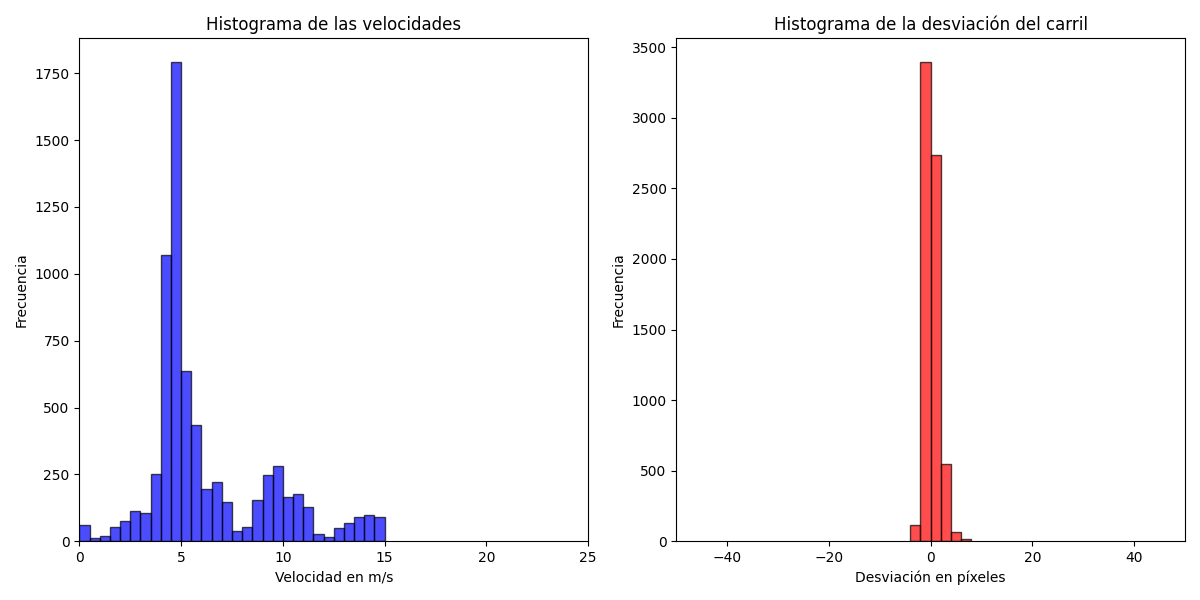
\includegraphics[width=0.45\textwidth]{figs/Diseño/discrete/train_env.png} \label{fig:pid_ajus}}
\hfill
\subfigure[Histogramas de un circuito no visto durante el entrenamiento.]{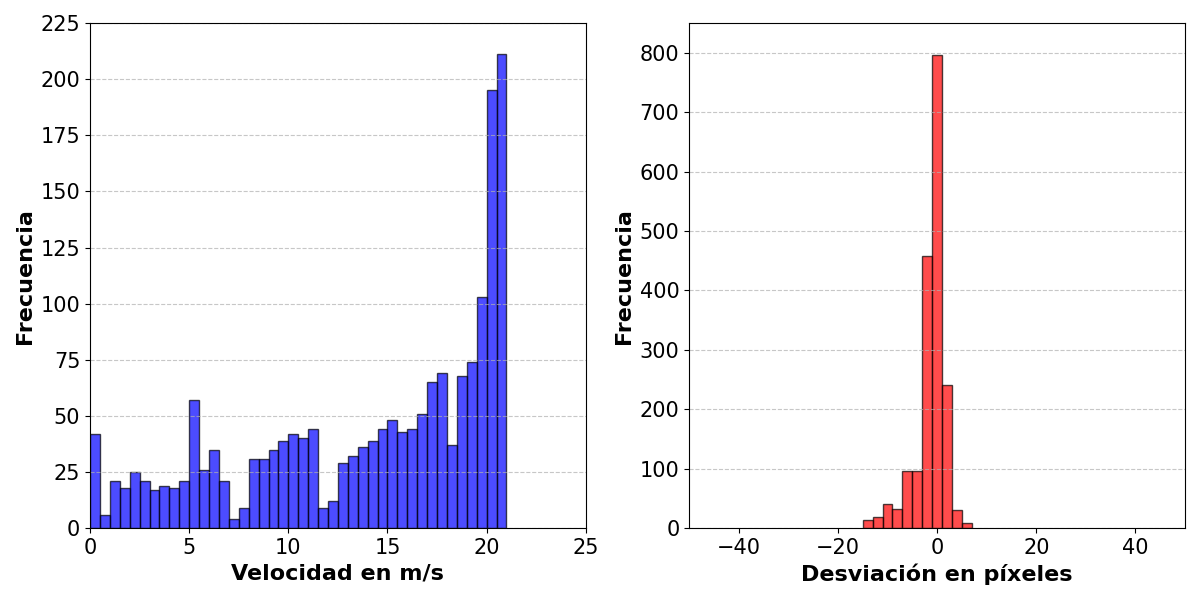
\includegraphics[width=0.45\textwidth]{figs/Diseño/discrete/no_train_env.png} \label{fig:pid_no_ajus}}
\caption{Comparativa de la velocidad y desviación del vehículo basado en \ac{DQN} en escenarios visto y no visto durante el entrenamiento.}
\label{fig:comparativa_dqn}
\end{figure}

Si comparamos este comportamiento con el obtenido con el controlador \ac{PID} \ref{fig:comparativa_pid}, vemos que, aunque el modelo basado en \ac{DQN} puede alcanzar velocidades superiores, generalmente es más lento. Esto se debe nuevamente a que el espacio de acciones es discreto y debemos definir pares fijos de acciones, el modelo no puede elegir el giro más conveniente en cada momento. No obstante, sí observamos una mejora significativa en la desviación respecto al centro del carril, especialmente en el escenario no ajustado o no visto durante el entrenamiento, el cual es el mismo en ambos casos. El modelo basado en \ac{DQN} es capaz de mantenerse dentro de los límites del carril con mayor precisión, garantizando una conducción más segura que el controlador \ac{PID}.

\subsection{Seguimiento de carril con \ac{PPO}}

El algoritmo \textit{Actor-Critic} es un tipo de algortimo en el que cada agente consta de dos elementos que aprenden de manera conjunta, cada uno con su propia red neuronal: \textit{actor}, encargado de aprender la política óptima, y \textit{critic}, responsable de aprender la función de valor y proporcionar una señal de refuerzo a la política. El algoritmo \ac{A2C} se forma a partir de la unión del actor y el critic y es una algoritmo \textit{on-policy}. \ac{PPO} es un algoritmo \textit{on-policy} que puede considerarse como una extensión de \ac{A2C}, cuyo objetivo principal es evitar el deterioro del rendimiento. En los algoritmos basados en políticas, ajustar la tasa de aprendizaje puede ser una labor complicada. Un valor pequeño puede llevar a entrenamientos prolongados sin alcanzar la solución óptima, mientras que uno grande puede causar un colapso en el rendimiento. Con el objetivo de resolver esto, \ac{PPO} introduce un objetivo sustituto que asegura una mejora monótona del rendimiento, evitando cambios drásticos y arriesgados en la política que puedan afectar negativamente al despeño. Para lograrlo, \ac{PPO} mide cuánto ha cambiado la política después de cada actualización, garantizando que esta diferencia sea no negativa en cada iteración, asegurando así una mejora continua en el rendimiento. Además, que impide que esta razón crezca o disminuya demasiado dentro de un umbral controlado por un hiperparámetro (\textit{clip\_range}) \cite{drl}. 

El objetivo sigue siendo conseguir un seguimiento de carril fluido y la mayor velocidad posible, pero esta vez usamos el algoritmo \ac{PPO} que permite un espacio de acciones continuo. Se emplea la misma lógica para la finalización de un episodio, sensores, \textit{fixed\_delta\_seconds} de 50ms y circuito de entrenamiento \ref{fig:mapa} que en el entorno anterior. Seguimos controlando dos elementos: el acelerador y el giro, permitimos el rango completo para el acelerador y limitamos el rango del giro.

\begin{code}[h]
\begin{lstlisting}[language=Python]
self._max_steer = 0.2
self.action_space = spaces.Box(
    low=np.array([0.0, -self._max_steer]),
    high=np.array([1.0, self._max_steer]),
    shape=(2,),
    dtype=np.float64
)
\end{lstlisting}
\caption[Espacio de acciones sigue-carril basado en \ac{PPO}]{Espacio de acciones sigue-carril basado en \ac{PPO}.}
\label{cod:acc_ppo}
\end{code}

Sin embargo, se han llevado a cabo algunos cambios en las observaciones. Se ha añadido la velocidad actual del vehículo al espacio de observaciones para mejorar la comprensión de la función de recompensa y, en lugar de cinco, ahora el modelo recibe diez puntos de cada línea del carril, como se muestra en la Figura \ref{fig:puntos_carril}, para mejorar la comprensión del mismo, sobre todo en las curvas.

En este caso, la función recompensa es más compleja y sigue el siguiente esquema:
\begin{enumerate}
    \item \textit{Comprobación de errores:} Primero se verifica si ha ocurrido un error, como pérdida del carril o choque contra elementos de la carretera. Si ocurre, se finaliza el episodio y se asigna una recompensa negativa.

    \item \textit{Normalización lineal de elementos:} Si no hay errores, se normalizan los elementos de los que depende la recompensa:
    \begin{itemize}
        \item \textit{Desviación:} Se limita el valor de la desviación al rango [-100, 100]. Se normaliza inversamente, donde una desviación de 0 tiene la mayor recompensa.
        \item \textit{Giro:} Para giros bruscos, la recompensa es nula. Para giros no bruscos, se normaliza inversamente considerando el rango [-0.14, 0.14], donde menores giros otorgan mayor recompensa.
        \item \textit{Acelerador:} Si las aceleraciones son bruscas en el rango [0.6, 1.0], la recompensa es nula. Para aceleraciones no bruscas en el rango [0.0, 0.6), si se supera la velocidad máxima, se normaliza inversamente, aceleración nula tiene mayor recompensa. En el caso contrario, se normaliza de forma que mayores aceleraciones otorgan mayor recompensa.
    \end{itemize}

    \item \textit{Asignación de pesos a los elementos:} Finalmente, se define el peso de cada elemento en la recompensa según los siguientes criterios:
    \begin{itemize}
        \item Si el giro o el acelerador son bruscos, tienen un peso muy elevado en la recompensa, mientras que los otros dos elementos tienen un peso mucho menor.
        \item Si se supera la velocidad máxima, el acelerador tiene mayor peso para intentar decelerar, penalizando también el giro debido a la alta velocidad, puesto que puede tener un gran impacto.
        \item Si el acelerador es bajo, en el rango [0.0, 0.5), se penalizan menos los giros grandes, facilitando las curvas al reducir la velocidad.
        \item Si el acelerador está en un rango alto [0.5, 0.6), se penalizan más los giros bruscos, enfocándose en zonas rectas o con giros leves.
    \end{itemize}
\end{enumerate}

\begin{code}[H]
\begin{lstlisting}[language=Python]
if error is None:
    # Deviation normalization
    r_dev = (MAX_DEV - abs(np.clip(self._dev, -MAX_DEV, MAX_DEV))) / MAX_DEV

    # Steer conversion
    limit_steer = 0.14
    if abs(self._steer) > limit_steer:
        r_steer = 0
    else:
        r_steer = (limit_steer - abs(self._steer)) / limit_steer

    # Throttle conversion
    limit_throttle = 0.6
    if self._throttle >= limit_throttle:
        r_throttle = 0
    elif self._velocity > self._max_vel:
        r_throttle = (limit_throttle - self._throttle) / limit_throttle
    else:
        r_throttle = self._throttle / limit_throttle

    # Set weight
    if r_steer == 0:
        w_dev, w_throttle, w_steer = 0.1, 0.1, 0.8
    elif r_throttle == 0:
        w_dev, w_throttle, w_steer = 0.1, 0.8, 0.1
    elif self._velocity > self._max_vel:
        w_dev, w_throttle, w_steer = 0.1, 0.65, 0.25
    elif self._throttle < 0.5:
        w_dev, w_throttle, w_steer = 0.65, 0.25, 0.1
    else:  # Throttle in range [0.5, 0.6)
        w_dev, w_throttle, w_steer = 0.6, 0.15, 0.25

    reward = w_dev * r_dev + w_throttle * r_throttle + w_steer * r_steer
else:
    reward = -40
\end{lstlisting}
\caption[Función de recompensa para sigue-carril basado en \ac{PPO}]{Función de recompensa para sigue-carril basado en \ac{PPO}.}
\label{cod:rew_ppo}
\end{code}

Al igual que en el entrenamiento anterior, el hiperparámetro \textit{n\_steps} fue clave a la hora de adquirir convergencia, también influyó el tamaño del lote, que inicialmente era demasiado pequeño. Con valores bajos del coeficiente de entropía, el agente aprendía siempre que las acciones límite maximizaban la recompensa, mientras que, con valores demasiado altos, no conseguía converger. Finalmente, estos fueron los hiperparámetros de entrenamiento utilizados:
\begin{code}[h]
\begin{lstlisting}[language=yaml]
policy: "MultiInputPolicy"
learning_rate: 0.0001
gamma: 0.85
gae_lambda: 0.9
n_steps: 512 # Numero de pasos a ejecutar antes de cada actualizacion
batch_size: 512 
ent_coef: 0.1 # Coeficiente de entropia
clip_range: 0.15 
n_timesteps: 4_000_000
\end{lstlisting}
\caption[Hiperparámetros de entrenamiento para el sigue-carril basado en \ac{PPO}]{Hiperparámetros de entrenamiento para el sigue-carril basado en \ac{PPO}.}
\label{cod:hiper_params_ppo}
\end{code}

\newpage

Al analizar los parámetros de entrenamiento de ambos algoritmos, podemos ver como con \ac{PPO} necesitamos la mitad de \textit{steps} que con \ac{DQN} para lograr un entrenamiento exitoso. Los entrenamientos con \ac{PPO} duraron aproximadamente unas veinte horas. En el siguiente gráfico, se muestran los datos de entrenamiento, donde se puede observar cómo se logra rápidamente la convergencia, pero se necesitan más \textit{steps} para alcanzar altas velocidades.
\begin{figure}[ht]
  \centering
  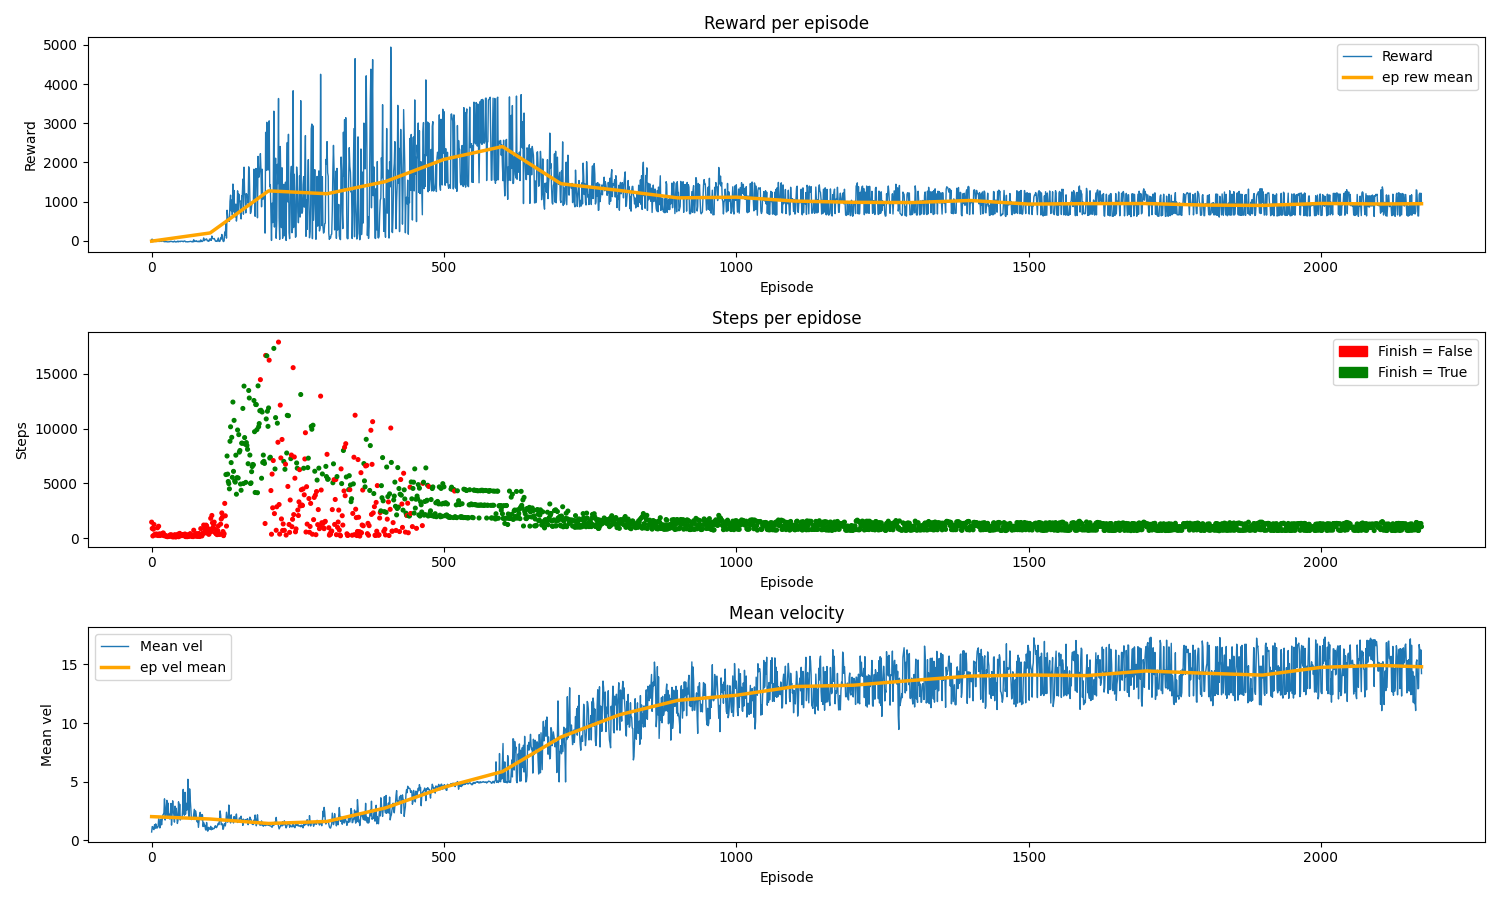
\includegraphics[width=13cm]{figs/Diseño/cont/train_ppo_carril.png}
  \caption{Gráficas de entrenamiento sigue-carril basado en \ac{PPO}.}
  \label{fig:train_ppo_carril}
\end{figure}

Debido a todos los inconvenientes con el coeficiente de entropía en  la exploración de acciones, también se desarrolló un programa para analizar la las frecuencia de las acciones tomadas durante el entrenamiento, cuyos resultados se presentan en el siguiente histograma.
\begin{figure}[ht]
  \centering
  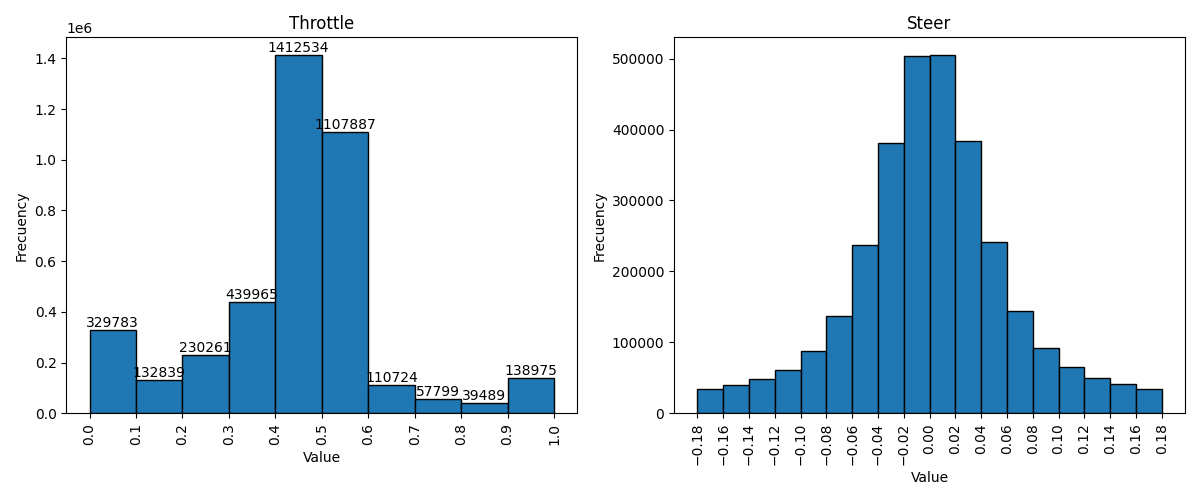
\includegraphics[width=11cm]{figs/Diseño/cont/actions_ppo_carril.png}
  \caption{Histogramas de acciones tomadas durante el entrenamiento sigue-carril basado en \ac{PPO}.}
  \label{fig:actions_ppo_carril}
\end{figure}

\newpage

En inferencia obtenemos muy buenos resultados tanto en circuitos utilizados durante el entrenamiento \footnote{\url{https://youtu.be/bZNfUwP14gc}} como en nuevos \footnote{\url{https://youtu.be/WRPLzKqJdto}}, incluso cambiando la ciudad en el simulador CARLA. A diferencia del modelo entrenado con \ac{DQN}, ahora si podemos elegir el giro exacto necesario en cada momento al disponer de un espacio de acciones continuo, lo que permite seguir el carril de forma más precisa y fluida. Además, se logran velocidades muy superiores, incluso superando los 20m/s. El modelo elige siempre aceleraciones en el rango [0.5, 0.6) combinadas con giros sutiles. Cabe destacar que, si eliminamos la parte del rango bajo del acelerador en la función recompensa, unificando ambos rangos en uno con los mismos pesos, el entrenamiento no logra converger, aunque al final siempre seleccione acciones en dentro del rango alto del acelerador.
\begin{figure}[ht]
  \centering
  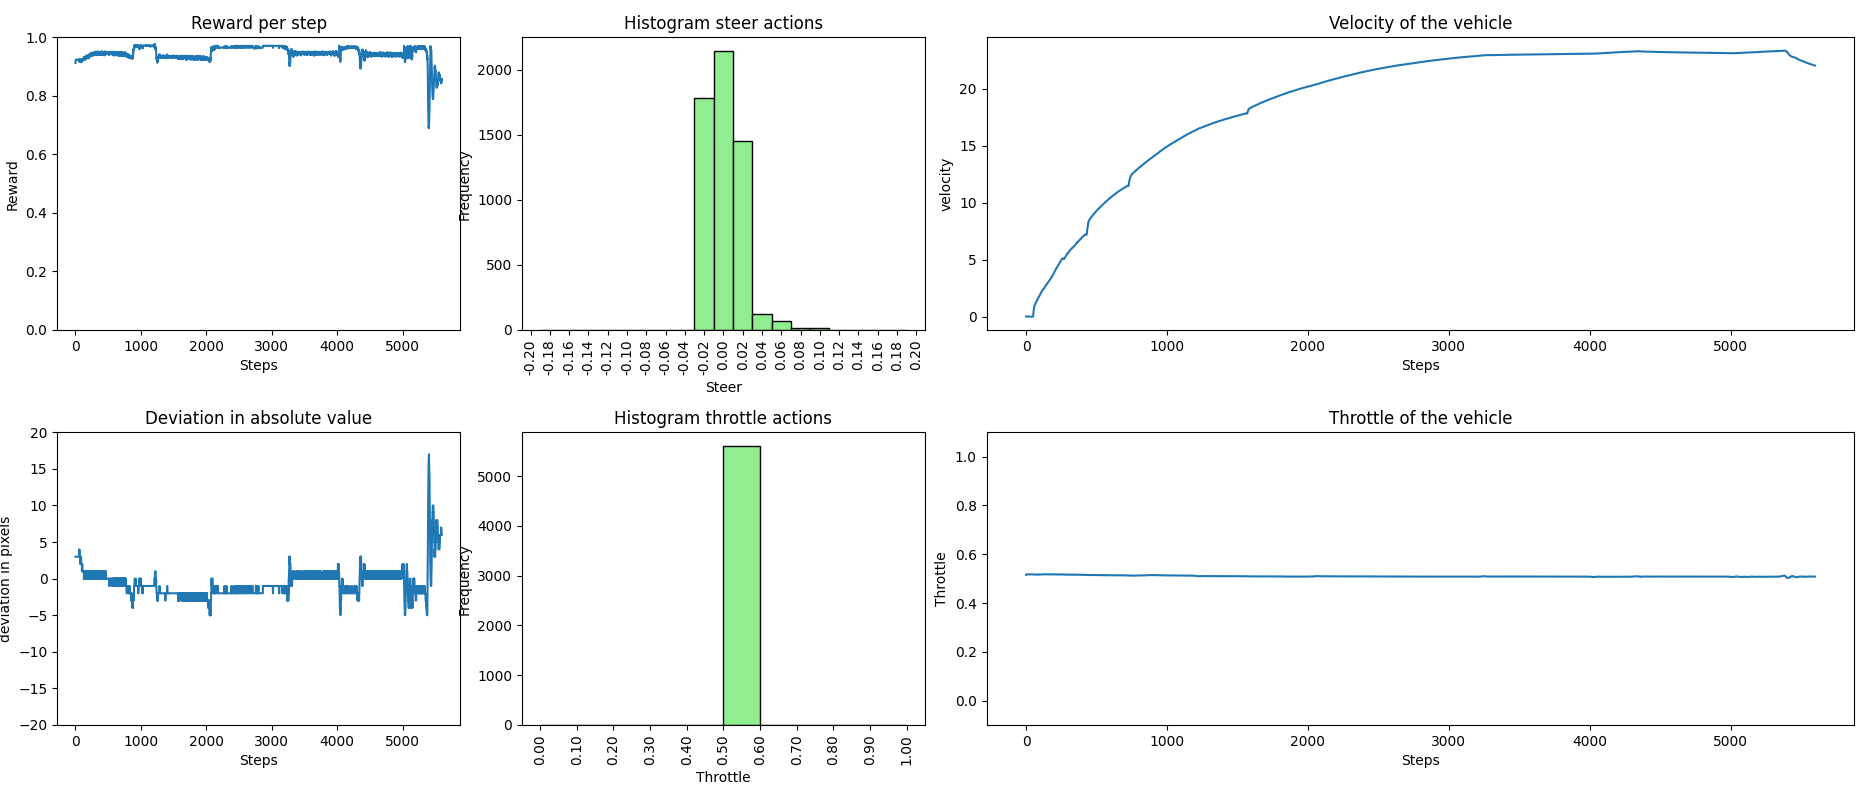
\includegraphics[width=15cm]{figs/Diseño/cont/inference.png}
  \caption{Gráfico de los datos recopilados durante inferencia del modelo sigue-carril con \ac{PPO}.}
  \label{fig:inference_ppo_carril}
\end{figure}

Recordemos, que los entrenamientos se han realizado utilizando la técnica de detección de carril \textit{ground thruth}. Si la cambiamos por la detección de carril basada en \ac{DL}, lo que incluye cambiar la posición de la cámara y, por tanto, la visión de percepción, seguimos obteniendo un seguimiento del carril fluido y conciso \footnote{\url{ https://youtu.be/8kOpXYqzIGM}} a altas velocidades.

\subsection{Control adaptativo con PPO}

Ahora el objetivo ha cambiado, el vehículo autónomo debe ser capaz de regular su velocidad en función del vehículo que tiene delante, controlado por el autopiloto de CARLA, además de seguir el carril. Para esta nueva funcionalidad, necesitamos añadir un nuevo sensor, el \ac{LiDAR}, cuyas observaciones son veinte puntos de la subzona frontal, como se muestra en la Figura \ref{fig:laser_front}. Mantenemos las mismas rutas de entrenamiento y resto de observaciones que en el apartado anterior. Seguimos utilizando el algoritmo de \ac{PPO} con el mismo espacio de acciones, ya que permite un control más fluido, preciso y un comportamiento más adaptativo al entorno. 

\begin{code}[h]
\begin{lstlisting}[language=Python]
self._num_points_laser = 20
self.observation_space[KEY_LASER] = spaces.Box(
	low=MIN_DIST_LASER - 1.0,
	high=MAX_DIST_LASER,
	shape=(self._num_points_laser,),
	dtype=np.float64
)
\end{lstlisting}
\caption[Definición de observación frontal del \ac{LiDAR}]{Definición de observación frontal del \ac{LiDAR}.}
\label{cod:obs_laser_front}
\end{code}

Un cambio clave respecto al modelo anterior es que, esta vez, hemos entrenado a 10 \ac{FPS} en lugar de 20 \ac{FPS}. A 20 \ac{FPS}, el agente no lograba un comportamiento adaptativo eficiente, sino un efecto de \textit{muelle}, acercándose demasiado al coche de delante, frenando bruscamente, alejándose y repitiendo el ciclo. En cambio, a 10 \ac{FPS}, se ha conseguido un comportamiento adaptativo más estable. Esto puede deberse a una reducción de ruido en las observaciones, los cambios en entorno y, por tanto, en las observaciones pueden ser más sutiles entre \textit{steps} consecutivos, permitiendo un mejor aprendizaje y compresión del escenario.

Para facilitar el aprendizaje del modelo, primero se realizado un entrenamiento exclusivamente para aprender a seguir el carril. Durante este entrenamiento, se ha \textit{congelado} la observación referente al \ac{LiDAR}, es decir, los puntos siempre tienen un valor predeterminado, el rango máximo del \ac{LiDAR} 19.5m. Los hiperparámetros de entrenamiento siguen siendo los mismos \ref{cod:hiper_params_ppo}, pero se ha reducido levemente el coeficiente de entropía a 0.08 para favorecer al explotación de acciones. En la función de recompensa, al haber cambiado la frecuencia de simulación, podemos eliminar la distinción entre acelerador bajo y alto en la definición de pesos, fusionándolos en un solo bloque.

\begin{code}[h]
\begin{lstlisting}[language=Python]
if r_steer == 0:
    w_dev, w_throttle, w_steer = 0.1, 0.1, 0.8
elif r_throttle == 0:
    w_dev, w_throttle, w_steer = 0.1, 0.8, 0.1
elif self._velocity > self._max_vel:
    w_dev, w_throttle, w_steer = 0.1, 0.65, 0.25
else:
    w_dev, w_throttle, w_steer = 0.6, 0.2, 0.2 # Follow Lane
\end{lstlisting}
\caption[Función de recompensa sigue-carril para el control adaptativo con \ac{PPO}]{Función de recompensa sigue-carril para el control adaptativo con \ac{PPO}.}
\label{cod:rew_carril_ppo_passing}
\end{code}

El modelo obtenido sigue el carril a la perfección \footnote{\url{https://youtu.be/flTo3YyFCHU}}, alcanzando velocidades superiores a 15m/s. De nuevo, se consigue una convergencia total rápidamente, pero seguimos necesitando un número elevado de \textit{steps} para adquirir altas velocidades. En inferencia, el modelo elige giros sutiles combinados con un valor del acelerador en el rango [0.47, 0.49].

\begin{figure}[ht]
  \centering
  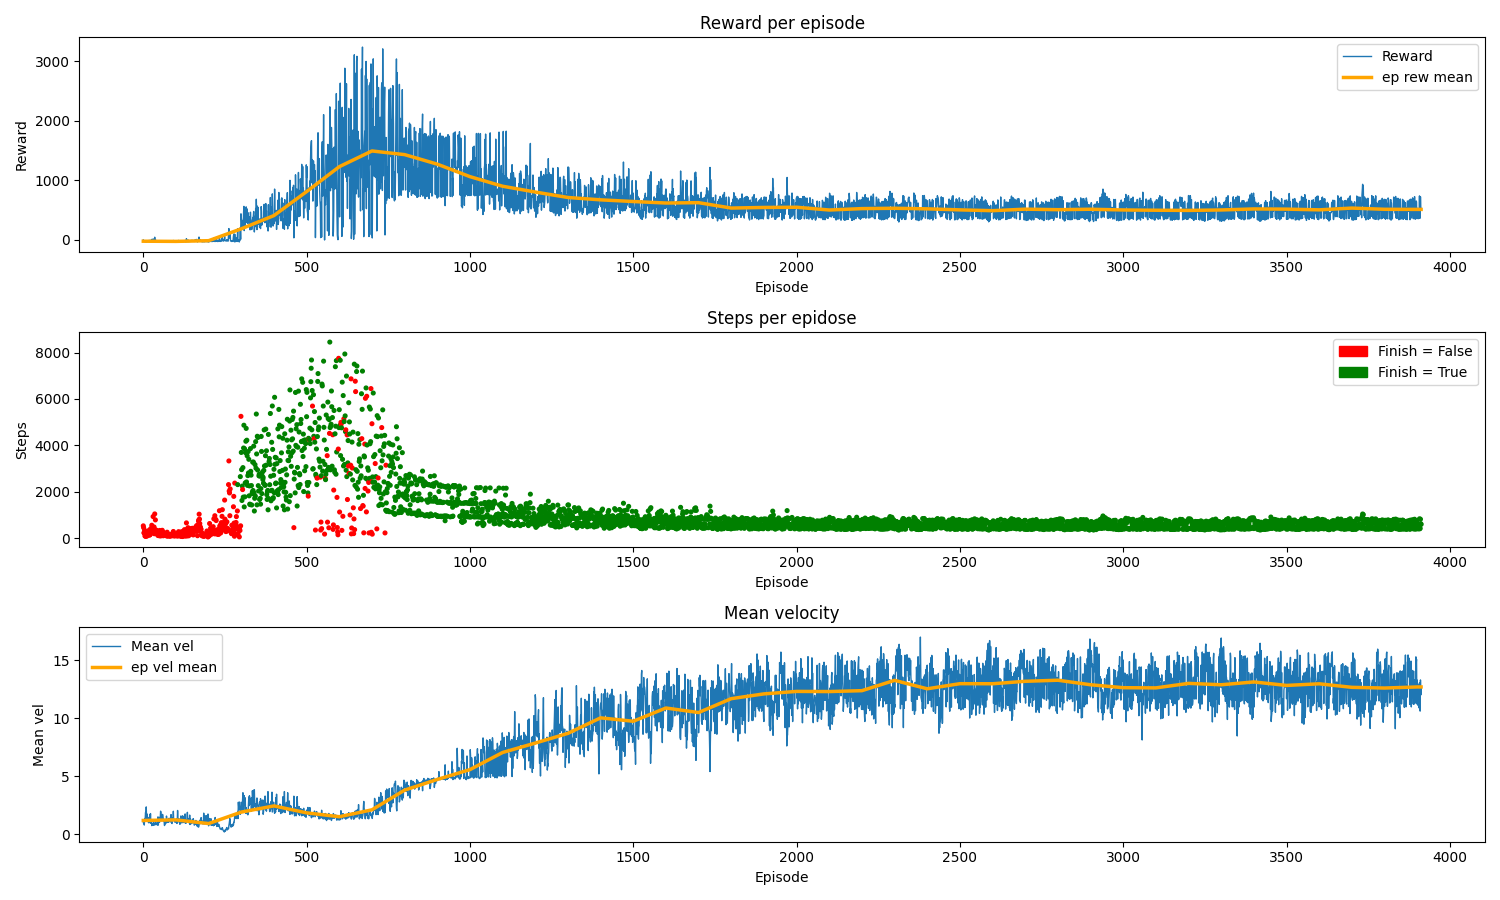
\includegraphics[width=8cm]{figs/Diseño/passing/train_base.png}
  \caption{Datos de entrenamiento sigue-carril para el control adaptativo con \ac{PPO}.}
  \label{fig:passing_train_base}
\end{figure}

\begin{figure}[ht]
  \centering
  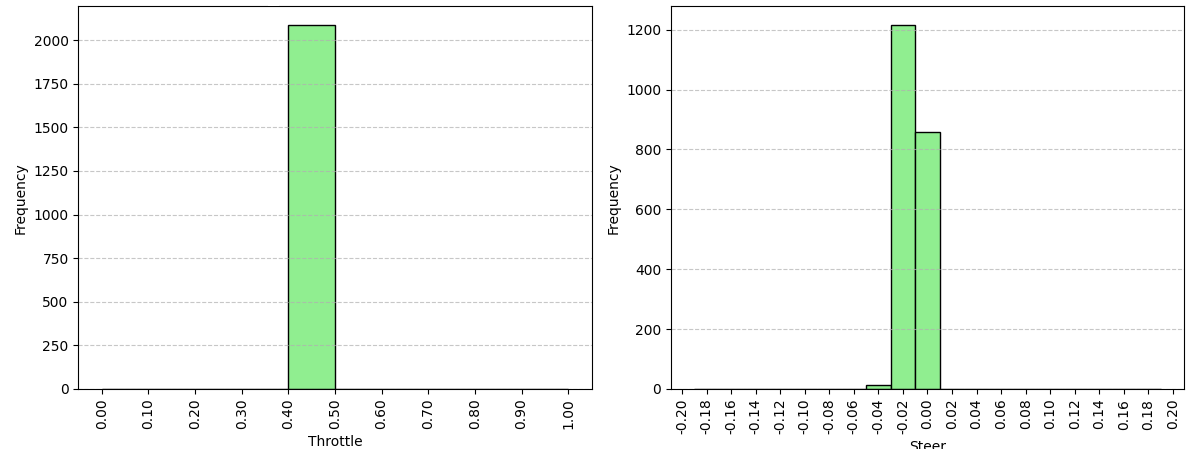
\includegraphics[width=10cm]{figs/Diseño/passing/actions_inference_base.png}
  \caption{Histogramas de acciones tomadas en inferencia durante el sigue-carril para el control adaptativo con \ac{PPO}.}
  \label{fig:passing_actions_inf_base}
\end{figure}

Ahora, necesitamos reentrenar el modelo sigue-carril para lograr un control adaptativo al tráfico. Durante este entrenamiento si activamos la observación del \ac{LiDAR} reales, cuya mínima distancia es incluida y normalizada en la función de recompensa con el fin de conseguir de que el vehículo autónomo sea capaz de circular detrás de un camión adaptándose a su velocidad. Si el coche está a una distancia menor de 4m, se provoca una excepción y se finaliza el episodio dando una recompensa negativa. Se penaliza aún más que salirse del carril, ya que es una acción más grave y que puede tener consecuencias fatales en el mundo real. Los pesos de la función de recompensa cuando vemos el vehículo delantero, dependen de la distancia: cuanto más próximo esté, mayor es la relevancia del \ac{LiDAR}, puesto que aumentan la criticidad de la situación.

\begin{code}[H]
\begin{lstlisting}[language=Python]
if error == None:
    # Deviation normalization, Steer conversion and Throttle conversion

    # LiDAR conversion
    if self._passing and not np.isnan(self._dist_laser):
        r_laser = (np.clip(self._dist_laser, MIN_DIST_LASER, MAX_DIST_LASER) - MIN_DIST_LASER) / (MAX_DIST_LASER - MIN_DIST_LASER)       
    else:
        r_laser = 0

    # Set weights
    # Filter inadequate actions
    elif r_laser != 0:
        if self._dist_laser <= 10:
            w_laser, w_steer, w_dev, w_throttle = 0.9, 0.0, 0.1, 0.0
        elif self._dist_laser <= 12:
            w_laser, w_dev, w_steer, w_throttle = 0.5, 0.45, 0.05, 0.0
        else:
            w_laser, w_dev, w_throttle, w_steer = 0.4, 0.5, 0.05, 0.05
    # Follow lane

    reward = w_dev * r_dev + w_throttle * r_throttle + w_steer * r_steer + w_laser * r_laser
else:
    if "Distance" in error:
        reward = -60
    else:
        reward = -40
\end{lstlisting}
\caption[Función de recompensa respecto al \ac{LiDAR} para control adaptativo con \ac{PPO}]{Función de recompensa respecto al \ac{LiDAR} para control adaptativo con \ac{PPO}.}
\label{cod:rew_ppo_passing}
\end{code}

Como el modelo ya sabe seguir el carril con una velocidad adecuada, no son necesarios tantos episodios de entrenamiento, por lo que hemos reducido el número de \textit{steps} a la mitad, dos millones. También se ha disminuido a la mitad el coeficiente de entropía 0.04, para evitar acciones aleatorias que puedan tener resultados fatales durante el episodio, como provocar una colisión con el camión.

La elección de velocidades del vehículo delantero fue crucial a la hora de lograr un comportamiento estable. Primeramente, se intentó estableciendo una velocidad constante durante un periodo de entre 100 y 450 \textit{steps} en el rango de [5, 10], escogiendo valores enteros y ambos de manera aleatoria. Sin embargo, se encontraron dos problemas:
  \begin{itemize}
        \item Para velocidades altas, el vehículo delantero se alejaba demasiado, sin que el agente pudiera verlo en ningún momento.
        \item El modelo se sobreajustaba a las velocidades bajas, limitándose a alcanzar velocidades máximas de 7 m/s.
    \end{itemize}
Para evitar el primer desafío, se diseñó un compartimento para que el camión delantero se parase si no estaba siendo visto por el agente, pero, aun así, el modelo resultante seguía siendo demasiado lento. Por ello, se modificó este comportamiento para que el camión solo se parase a distancias superiores 30 metros, con la diferencia de distancia entre ambos vehículos se obtuvo directamente del simulador CARLA. De esta forma, garantizamos que el modelo pueda ver al vehículo delantero en todas las velocidades, a la vez que se generen ocasiones en las que no lo vea, lo que ayuda a evitar el sobreajuste del modelo y a mantener las altas velocidades.

\begin{code}[H]
\begin{lstlisting}[language=Python]
if self._count_random % self._random_steps == 0 and self._count_random != 0:
	self._target_vel =  random.randint(5, 10)
	self._random_steps = random.randint(100, 450)
	self._count_random = 0

if loc_ego.distance(self._front_vehicle.get_location()) > 30:
	self._tm.set_desired_speed(self._front_vehicle, 0)  # km/h
else:
	self._tm.set_desired_speed(self._front_vehicle, self._target_vel * 3.6)
	self._count_random += 1
\end{lstlisting}
\caption[Función de recompensa respecto al \ac{LiDAR} para control adaptativo con \ac{PPO}]{Función de recompensa respecto al \ac{LiDAR} para control adaptativo con \ac{PPO}.}
\label{cod:rew_ppo_passing}
\end{code}

El siguiente histograms muestra el número de \textit{steps} durante los que el agente ha observado las diferentes velocidades, así como aquellos en los que no ha detectado el camión delantero durante el reentrenamiento. La fracción de veces que ha visto el camión muy superior a la que no lo ve, pero debemos recordar que en el entrenamiento base de seguimiento de carril no ha visto un vehículo delante en ninguno de los episodios.
\begin{figure}[ht]
  \centering
  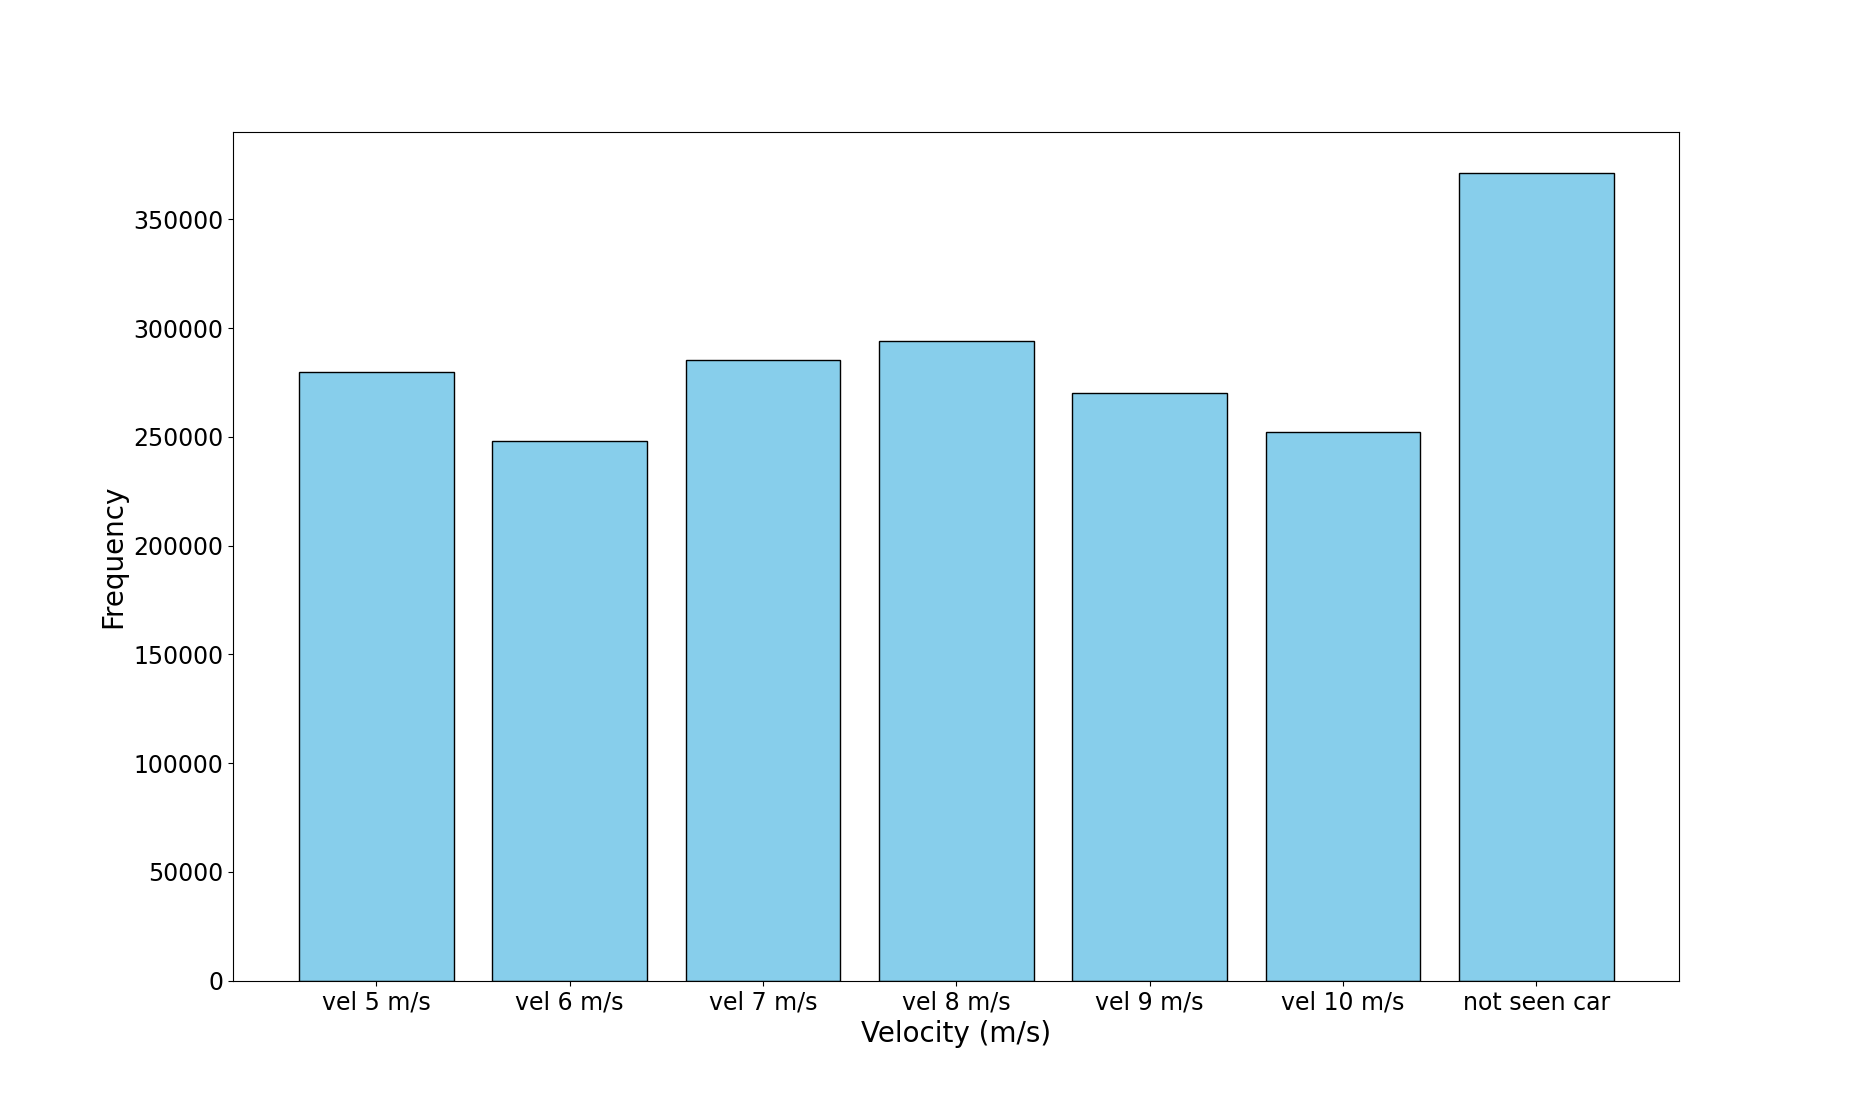
\includegraphics[width=9cm]{figs/Diseño/passing/velocities.png}
  \caption{Histograma de velocidades vistas durante el entrenamiento para el control adaptativo con \ac{PPO}.}
  \label{fig:velocities}
\end{figure}

\newpage

Aunque no se alcanza una convergencia total como en entrenamientos anteriores, podemos decir que el modelo sí converge, ya que la recompensa promedio de los episodios aumenta de manera a lo largo del proceso de entrenamiento. Esto sugiere que, a pesar de los episodios no finalizados, el modelo está mejorando gradualmente su desempeño y aprendiendo de manera efectiva. 
\begin{figure}[ht]
  \centering
  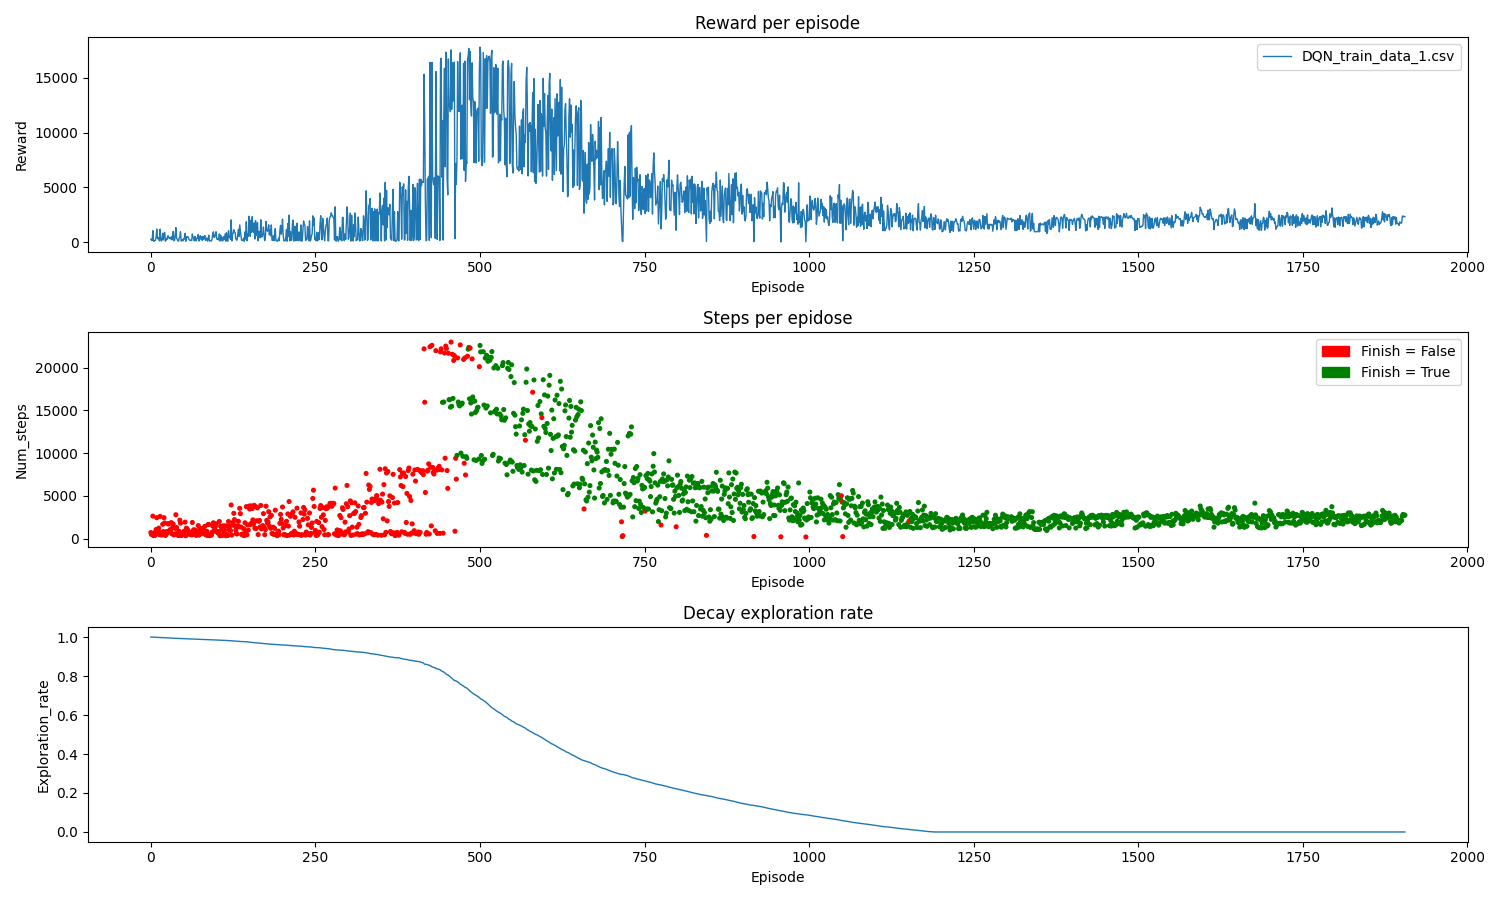
\includegraphics[width=13cm]{figs/Diseño/passing/train.png}
  \caption{Datos de reentrenamiento control adaptativo con \ac{PPO}.}
  \label{fig:velocities}
\end{figure}

En la fase de inferencia, se obtienen buenos resultados a distintas velocidades, tanto altas como bajas, y se sigue manteniendo el seguimiento preciso del carril. La velocidad del coche delantero influye en la distancia de estabilización, es decir, la separación con la que el coche autónomo se mantiene del camión. A mayor velocidad, mayor es esta distancia de seguridad, lo que es lógico y necesario en un entorno real. También se lograr resultados satisfactorios en circuitos no vistos durante el entrenamiento, incluso cambiando de ciudad en CARLA \footnote{\url{https://youtu.be/ieMD1wqqEaY}}. 

Los siguientes diagramas muestran los datos de inferencia recolectados cuando el coche delantero circula a 9 m/s y 5 m/s, respectivamente. Podemos verificar la teoría anterior analizando los histogramas de distancias del \ac{LiDAR}: si el vehículo delantero se desplaza a 9 m/s \footnote{\url{https://youtu.be/mN0Y2q6ny5w}}, el agente mantiene una distancia de unos 14-15 metros; mientras que si circula a 5 m/s \footnote{\url{https://youtu.be/Gvh9ZS0Sizc}}, la distancia se estabiliza en torno a los 13 metros. En cuanto a la velocidad, esta aumenta rápidamente al inicio y luego se estabiliza en un valor cercano al del coche delantero, podemos observar pequeñas fluctuaciones que indican ajustes constantes para mantener la distancia de seguridad. Esto también se refleja en el comportamiento del acelerador, donde la mayoría de las acciones se concentran en el rango [0.4, 0.5], lo que sugiere que el vehículo mantiene una aceleración constante en lugar de realizar ajustes bruscos, logrando así una conducción más suave.

\begin{figure}[ht]
  \centering
  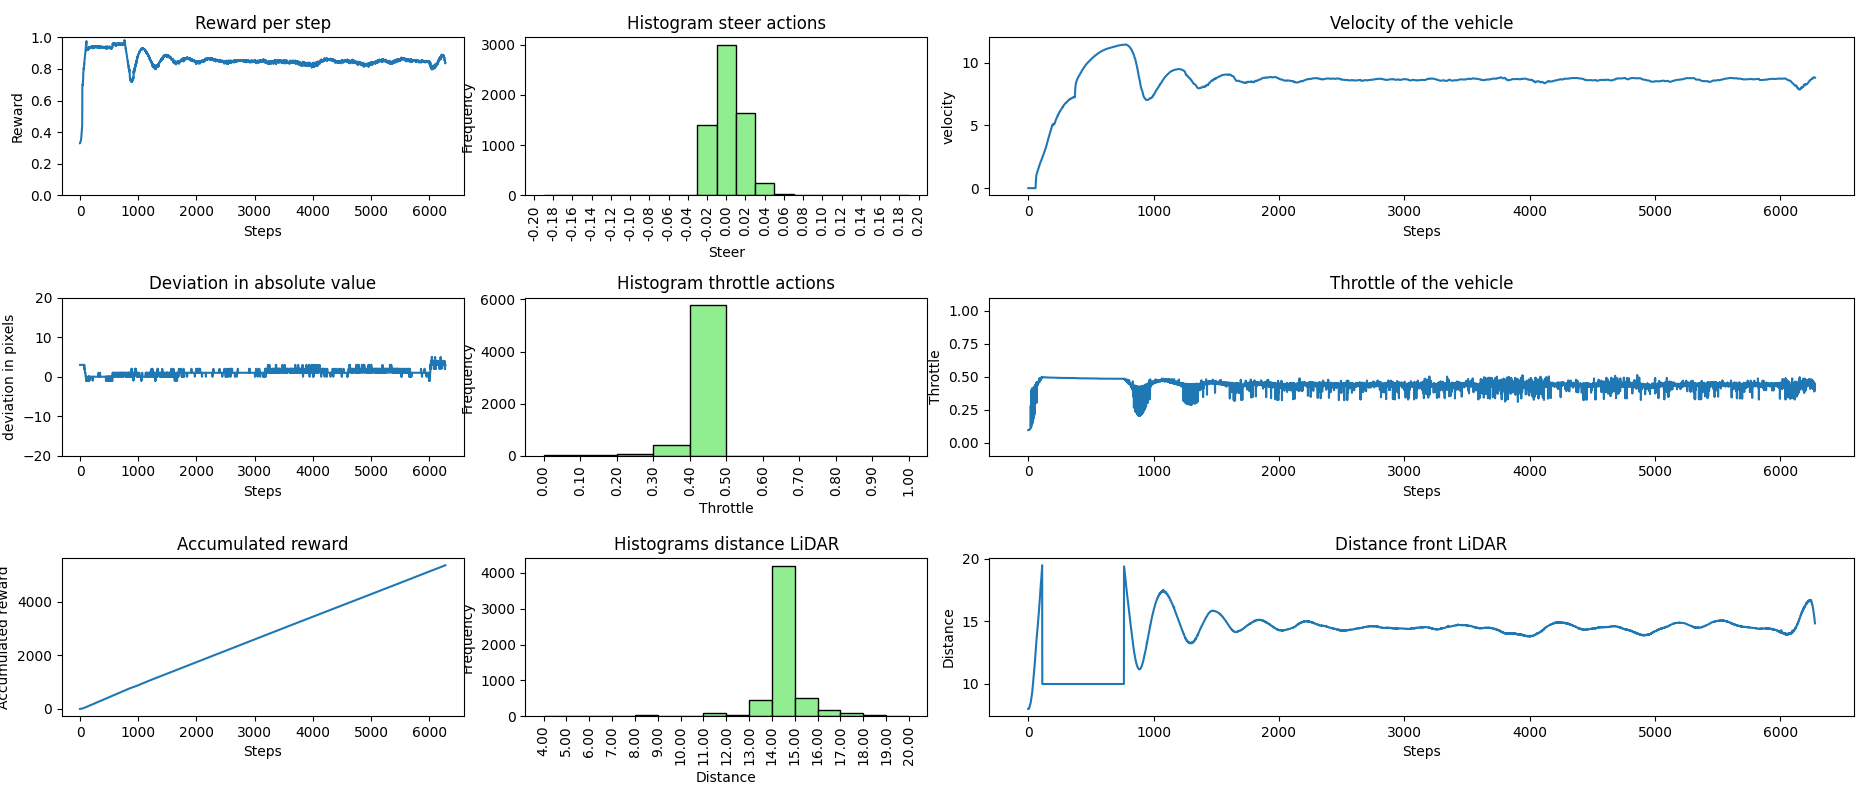
\includegraphics[width=14cm]{figs/Diseño/passing/inference_9.png}
  \caption{Datos de inferencia del control adaptativo con \ac{PPO}, donde el vehículo delantero mantiene una velocidad de 9m/s.}
  \label{fig:infrence_passing}
\end{figure}
\begin{figure}[ht]
  \centering
  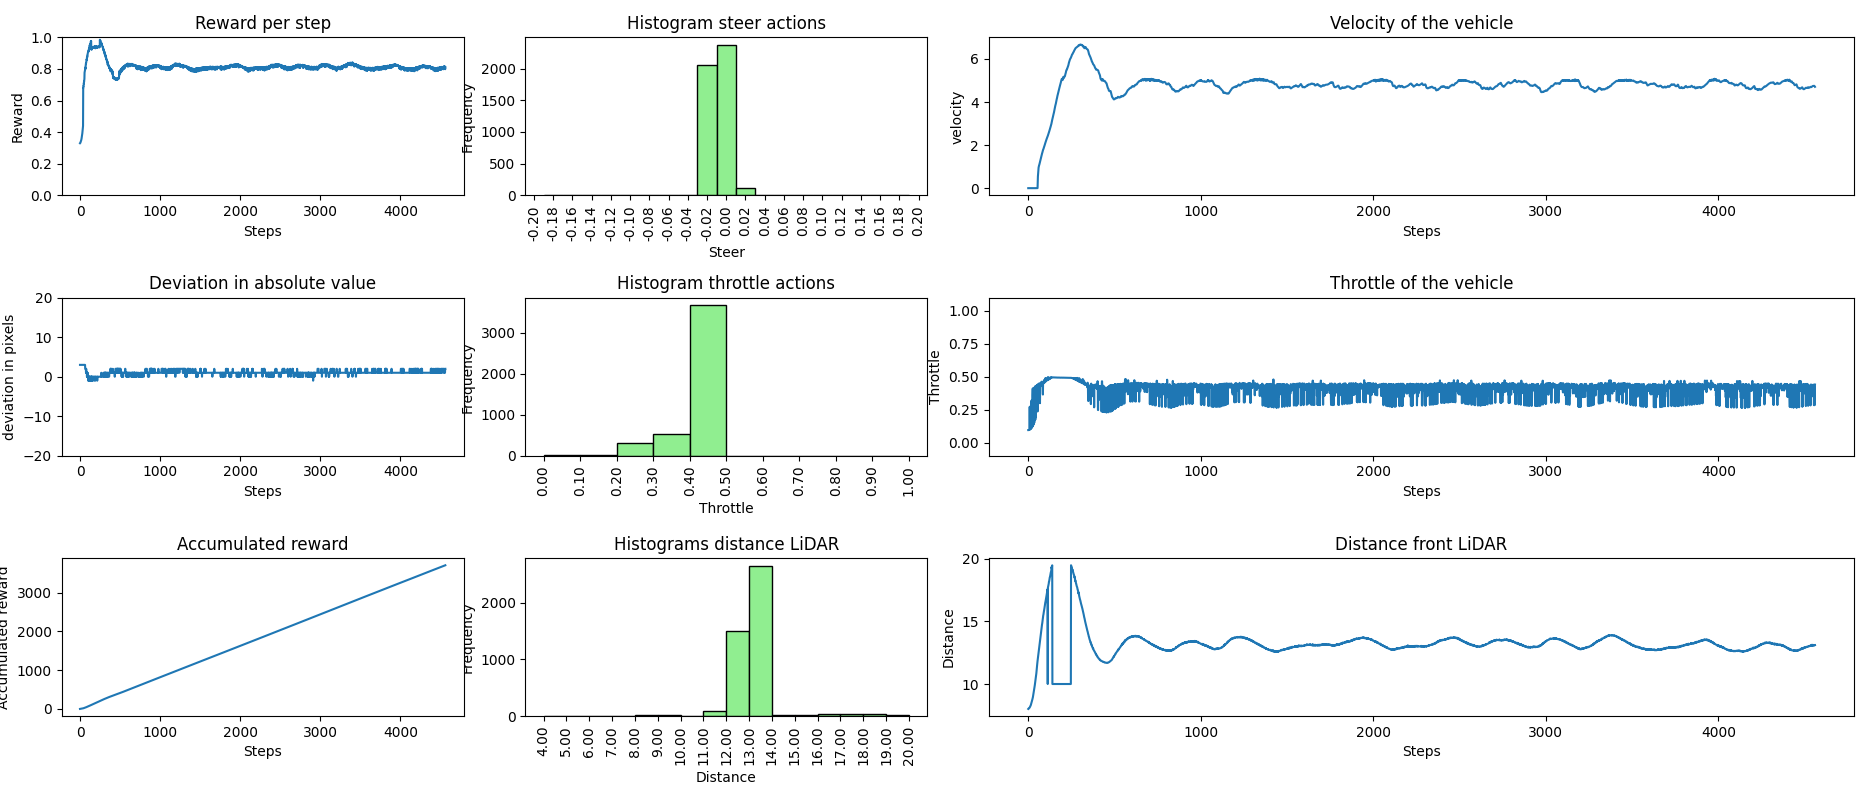
\includegraphics[width=14cm]{figs/Diseño/passing/inference_5.png}
  \caption{Datos de inferencia del control adaptativo con \ac{PPO}, donde el vehículo delantero mantiene una velocidad de 5m/s.}
  \label{fig:infrence_passing}
\end{figure}

\subsection{Maniobra de adelantamiento con PPO}

En este apartado se describe como se ha alcanzo el objetivo final, realizar una maniobra de adelantamiento completa. Cuando se haya visualizado el vehículo delantero a menos de 15 metros, se inicia el cambio de carril a la izquierda y, una vez ya no detectemos el vehículo en la parte derecha del \ac{LiDAR}, el coche autónomo vuelve al carril original. Para ello, es necesario añadir nuevas observaciones al modelo, tanto referentes a la zona derecha del \ac{LiDAR}, como a la segmentación de la calzada. Estas son todas las observaciones que recibe el modelo:
\begin{itemize}
\item Velocidad del propio agente, es decir, del \textit{Ego Vehicle}.
\item Desviación del carril.
\item Centro de masas del carril.
\item Área del carril.
\item 10 puntos de la línea de carril izquierda.
\item 10 puntos de la línea del carril derecha.
\item 10 puntos de la subzona frontal del \ac{LiDAR}.
\item 10 puntos de la subzona frontal derecha del \ac{LiDAR}.
\item 10 puntos de la subzona derecha del \ac{LiDAR}.
\item 10 puntos de la subzona trasera derecha del \ac{LiDAR}.
\item Centro de masas de la calzada.
\item Área de la calzada.
\item 16 puntos del límite izquierdo de la calzada.
\item 16 puntos del límite derecho de la calzada.
\end{itemize}

\begin{figure}[ht]
  \centering
  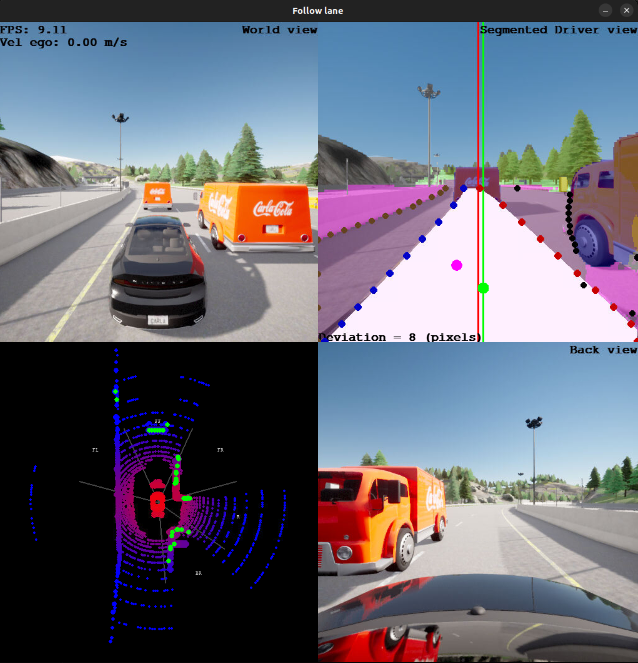
\includegraphics[width=11cm]{figs/Diseño/overtaken/obs.png}
  \caption{Observaciones en el modelo de adelantamiento con \ac{PPO}.}
  \label{fig:obs_overtaken}
\end{figure}

Es necesario analizar todas las subzonas del \ac{LiDAR}, excluyendo la del lado izquierdo, para determinar cuándo es seguro regresar al carril inicial durante un adelantamiento. Para intentar tener en cuenta solo información que concierne a la conducción, se ha realizado un filtrado por distancia dependiendo de la subzona, ya que, por ejemplo, necesitamos más rango del en la zona frontal del \ac{LiDAR} que en la lateral. De esta manera, nos aseguramos que el modelo recibe solo puntos dentro de la carreta. Los filtros de distancia aplicados según la zona son los siguientes:
\begin{itemize}
\item \textit{Front}: no aplicamos filtro distancia, por lo que disponemos del rango total del \ac{LiDAR}, como se muestra en la Figura \ref{fig:laser_front}.
\item \textit{Right-front}: nos quedamos con distancias iguales o menores a 7m.
\item \textit{Right}: filtrado por distancia de 6m.
\item \textit{Right-back}: filtramos distancias inferiores a 9m.
\end{itemize}

\begin{figure}[ht]
\centering
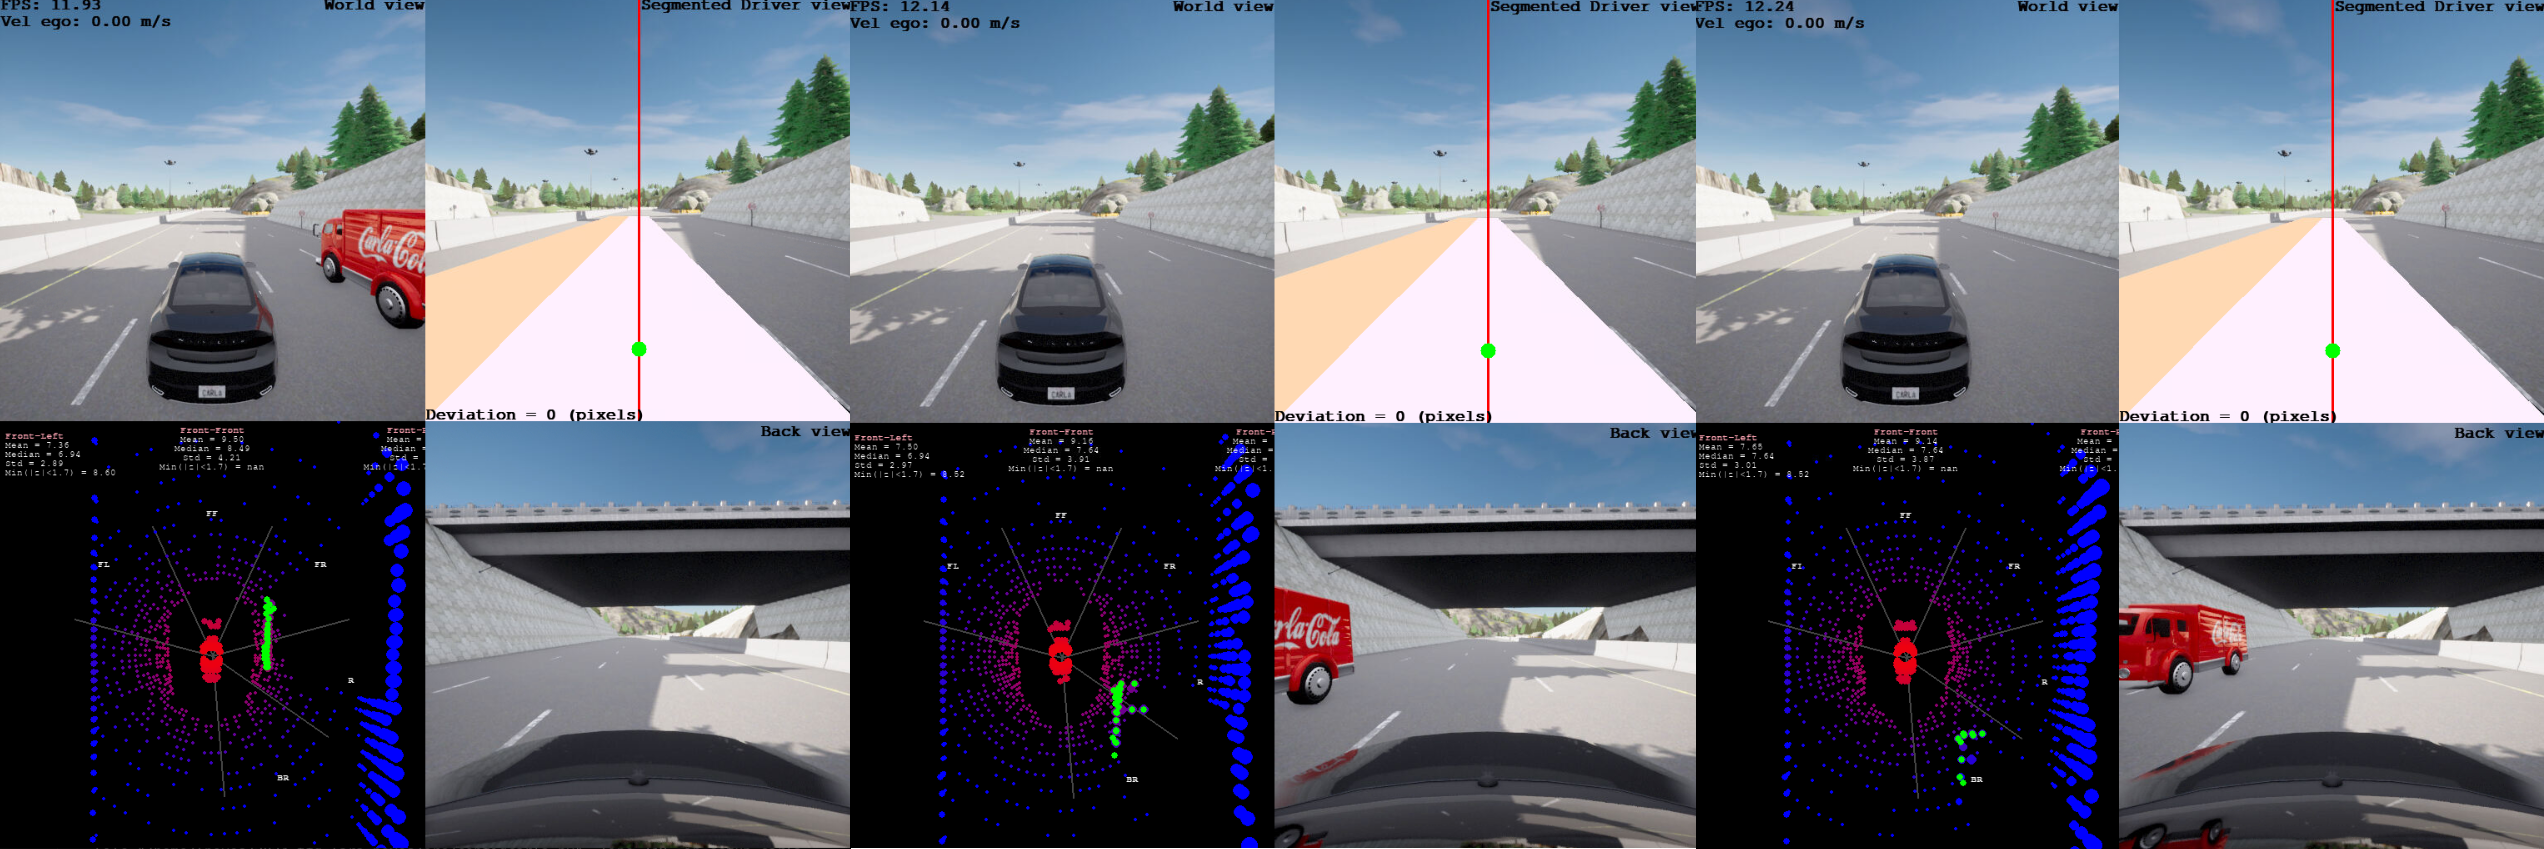
\includegraphics[width=11cm]{figs/Diseño/lidar/laser_right.png}
\caption{Filtrado del \ac{LiDAR} zona derecha.}
\label{fig:laser_right}
\end{figure}

Al igual que para el control adaptativo, se realiza un primer entrenamiento para conseguir un modelo capaz de seguir el carril de manera precisa y a altas velocidades. Se ha entrenado a 9 \ac{FPS}, pero esta vez no porque se obtuviera mejoren resultados, sino porque en inferencia se logra ir como máximo a unos 10 \ac{FPS}. Se han reutilizado tanto la función recompensa \ref{cod:rew_carril_ppo_passing} como los hiperparámetros de entrenamiento del modelo sigue-carril para el control adaptativo. Durante este entrenamiento, a diferencia del modelo anterior, no desactivamos las observaciones no relavaste para el seguimiento de carril, el agente recibe constantemente observaciones reales del carril, \ac{LiDAR} y segmentación de la calzada. El circuito usado durante todos entrenamientos, dispone de tres rutas en los que el coche va por el carril más a la derecha en una de ellas y, en las otras dos, por los carriles centrales. Para fomentar la visualización de todos los posibles estados en la calzada, se ha añadido una nueva ruta en la que el vehículo autónomo circula por el carril más a la izquierda, como se puede ver en la Figura \ref{fig:obs_overtaken}. Los resultados han sido…
